\documentclass[11pt]{article}
\usepackage[letterpaper,margin=1in]{geometry}
\usepackage{amsmath,amssymb,amsthm,mathtools,bm}
\usepackage{graphicx}
\usepackage{enumitem}
\usepackage[hidelinks]{hyperref}
\usepackage[T1]{fontenc}
\usepackage{lmodern}
\usepackage{xcolor}
\newcommand{\redstarfootnote}[1]{%
  \textcolor{red}{\textsuperscript{*}}%
  \begingroup
  \renewcommand{\thefootnote}{\textcolor{red}{*}}%
  \footnotetext{\textcolor{red}{#1}}%
  \endgroup
}
\usepackage[normalem]{ulem}
\newcommand{\rev}[1]{\textcolor{red}{#1}}
\newcommand{\del}[1]{\textcolor{red}{\sout{#1}}}
\newenvironment{revision}{\color{red}}{}
\newcommand{\bAd}{\mathbf{Ad}}
\newcommand{\bad}{\mathbf{ad}}
\newcommand{\JopL}{\mathcal J_l}
\newcommand{\JopR}{\mathcal J_r}
\newcommand{\JL}{J_l}
\newcommand{\JR}{J_r}
\newcommand{\Exp}{\operatorname{Exp}}
\newcommand{\Log}{\operatorname{Log}}
\setlength{\parindent}{1.5em}
\setlength{\parskip}{0.2em}
\newcommand{\SO}{\mathrm{SO}}
\newcommand{\SE}{\mathrm{SE}}
\newcommand{\so}{\mathfrak{so}}
\newcommand{\se}{\mathfrak{se}}
\newcommand{\gfrak}{\mathfrak g}
\newcommand{\Ad}{\operatorname{Ad}}
\newcommand{\ad}{\operatorname{ad}}
\newcommand{\id}{\operatorname{id}}
\newcommand{\tr}{\operatorname{tr}}
\newcommand{\pr}{\operatorname{pr}}
\newcommand{\vers}{\operatorname{vers}}
\newcommand{\R}{\mathbb R}
\newcommand{\calB}{\mathcal B}
\newcommand{\eps}{\varepsilon}
\newcommand{\proofbox}{\hfill$\square$}
\newcounter{paperlemma}
\newcounter{papertheorem}
\newcounter{paperproposition}
\newcounter{paperremark}
\newcounter{paperexample}
\renewcommand{\thepaperlemma}{\arabic{paperlemma}}
\renewcommand{\thepapertheorem}{\arabic{papertheorem}}
\renewcommand{\thepaperproposition}{\arabic{paperproposition}}
\renewcommand{\thepaperremark}{\arabic{paperremark}}
\renewcommand{\thepaperexample}{\arabic{paperexample}}
\newcommand{\paperlemma}[3]{\refstepcounter{paperlemma}\par\medskip\noindent\textbf{Lemma \thepaperlemma\ (#1).}\label{#2} \textit{#3}\par}
\newcommand{\papertheorem}[3]{\refstepcounter{papertheorem}\par\medskip\noindent\textbf{Theorem \thepapertheorem\ (#1).}\label{#2} \textit{#3}\par}
\newcommand{\paperproposition}[2]{\refstepcounter{paperproposition}\par\medskip\noindent\textbf{Proposition \thepaperproposition.}\label{#1} \textit{#2}\par}
\newcommand{\paperremark}[2]{\refstepcounter{paperremark}\par\medskip\noindent\textbf{Remark \thepaperremark#1.}\label{#2}\ }
\newcommand{\paperexample}[2]{\refstepcounter{paperexample}\par\medskip\noindent\textbf{Example \thepaperexample#1.}\label{#2}\ }
\title{Proportional Derivative (PD) Control on the Euclidean Group}
\author{F. Bullo \qquad R. M. Murray\\[0.5em]
Division of Engineering and Applied Science\\
California Institute of Technology\\
Pasadena, CA 91125}
\date{CDS Technical Report 95-010\\August 11, 1995}
\begin{document}
\maketitle

\begin{abstract}
In this paper we study the stabilization problem for control systems defined on $\SE(3)$ (the special Euclidean group of rigid-body motions) and its subgroups. Assuming one actuator is available for each degree of freedom, we exploit geometric properties of Lie groups (and corresponding Lie algebras) to generalize the classical proportional derivative (PD) control in a coordinate-free way. For the $\SO(3)$ case, the compactness of the group gives rise to a natural metric structure and to a natural choice of preferred control direction: an optimal (in the sense of geodesic) solution is given to the attitude control problem. In the $\SE(3)$ case, no natural metric is uniquely defined, so that more freedom is left in the control design. Different formulations of PD feedback can be adopted by extending the $\SO(3)$ approach to the whole of $\SE(3)$ or by breaking the problem into a control problem on $\SO(3)\times\R^3$. For the simple $\SE(2)$ case, simulations are reported to illustrate the behavior of the different choices. We also discuss the trajectory tracking problem and show how to reduce it to a stabilization problem, mimicking the usual approach in $\R^n$. Finally, regarding the case of underactuated control systems, we derive linear and homogeneous approximating vector fields for standard systems on $\SO(3)$ and $\SE(3)$.
\end{abstract}

\noindent\textbf{Key words and phrases.} PD control, Euclidean group, nonlinear control, workspace control.

\noindent Funding for this research was provided in part by NSF grant CMS-9502224. An abbreviated version of this paper can be found in the Proc. of the 1995 European Control Conference. Work performed in part while author was with the Dipartimento di Ingegneria Elettronica, Universit\`a di Padova, Italy.

\tableofcontents

\section{Introduction}\label{sec:introduction}
We here consider the problem of controlling a (mechanical) system whose configuration space is a matrix Lie group: we focus on second order systems and attempt to generalize the standard notion of proportional derivative feedback. One large class of applications which motivates this work is workspace control of robotic manipulators, where the end-effector configuration is naturally embedded in $\SE(3)$ (see \cite{26} for a description of the workspace control problem and traditional solutions). While local solutions are easily obtained, we hope that a more geometric approach will yield advantages similar to those afforded by the geometric approach to kinematics in \cite{26}.

Historically, nonlinear control systems defined on Lie groups have received considerable attention in the literature: early work by Brockett \cite{5,7}, Jurdjevic and Sussman \cite{15}, and others has served as motivation for more recent contributions by Walsh, Sarti, Sastry and Montgomery \cite{29,32}, Leonard and Krishnaprasad \cite{20,21}, and Crouch and Silva Leite \cite{10}, to name a few. Early works concentrated on problem formulation and controllability issues, while the more recent papers mainly consider constructive controllability: how to generate a feasible trajectory between two (or more) points on the configuration manifold given a limited number of actuators.

Our approach in this paper is somewhat different. We concentrate on the problems of stabilization and trajectory tracking in the fully actuated case, where one actuator is available for each degree of freedom in the system. This is traditionally the situation for problems in robotic manipulation, satellite reorientation and 6 degree of freedom underwater vehicles. We attempt to exploit the geometric properties of Lie groups and to generalize the classical proportional plus derivative feedback (PD) used for control of simple mechanical systems in $\R^n$. For the case of compact Lie groups, such as $\SO(3)$, our results are completely general. For the non-compact case, we consider only control systems on $\SE(3)$ and on its subgroups, since those are the main systems of interest in our applications.

The paper is organized as follows. In Section~\ref{sec:systems-lie-groups}, we introduce basic and new results on systems defined on Lie groups. Section~\ref{sec:pd-so3} shows stabilization results for the compact case and in particular for $\SO(3)$. Section~\ref{sec:pd-se3} considers the $\SE(3)$ case, a non-compact, non-semisimple group. Different metrics lead to different control laws. These results are then generalized to the trajectory tracking case in Section~\ref{sec:trajectory-tracking}. In Section~\ref{sec:linear-homogeneous} we deal with underactuated control systems and we show how the algebraic tools developed in the previous sections lead to simple linear and homogeneous approximations for standard systems on the Euclidean group. Section~\ref{sec:summary-conclusions} discusses the results.

\section{Systems on Lie groups}\label{sec:systems-lie-groups}
We here review the notations and give some algebraic results on Lie groups and on dynamical systems evolving on Lie groups. For a comprehensive introduction in the context of robotics, see \cite[Appendix A]{26}.

\subsection{Basic definitions and results}\label{subsec:basic-definitions}
In the following we focus our attention on the matrix Lie group $\SE(3)$ and its proper subgroups, even though most of the results hold more generally.\footnote{We will denote with $G$ the generic Lie group ($\gfrak$ being its Lie algebra), while for specific results we will refer to $\SE(3)$, $\SO(3)$ etc.} Let $G\subset\SE(3)$ be a matrix Lie group and $\gfrak\subset\se(3)$ its Lie algebra. A dynamical system with state $g\in G$ evolves following
\begin{equation*}
\dot g=gV^b=V^s g,\qquad V^b,V^s\in\gfrak,\tag{2.1}\label{eq:2.1}
\end{equation*}
where we can express the velocity in body ($V^b$) or in spatial frame ($V^s$). To keep the notation consistent, we will use lower case symbols for elements in the group and upper case for elements in the algebra. Since the system $\dot g=gV^b$ is invariant under left multiplication by constant matrices, we call it \emph{left invariant}; correspondingly $\dot g=V^s g$ is said to be \emph{right invariant}. For all $g\in G$ and all $X,Y\in\gfrak$, the adjoint map $\Ad_g$ and the matrix commutator $\ad_X$ are defined as
\begin{equation*}
\Ad_g(Y)=gYg^{-1},\qquad \ad_X(Y)=[X,Y]=XY-YX.
\end{equation*}

\begin{revision}
After choosing a basis $\mathcal E=(E_1,\ldots,E_n)$ of $\gfrak$, write $X=x^\wedge$ and $Y=y^\wedge$. We use boldface for the matrices representing the linear maps $\Ad_g$ and $\ad_X$ in these coordinates. Thus
\[
\bigl(\Ad_g(Y)\bigr)^\vee=\bAd_g\,y,
\qquad
\bigl(\ad_X(Y)\bigr)^\vee=\bad_x\,y,
\]
with
\[
\boxed{
\bAd_g:=\vee\circ\Ad_g\circ\wedge,
\qquad
\bad_x:=\vee\circ\ad_{x^\wedge}\circ\wedge.
}
\]
\end{revision}

On $\SE(3)$ and $\se(3)$ we represent a group element $g=(R,p)\in\SO(3)\times\R^3$ and a velocity $V=(\widehat\omega,v)\in\so(3)\times\R^3$ using homogeneous coordinates,

\begin{equation*}
g=\begin{bmatrix}R&p\\0&1\end{bmatrix},\qquad
V=\begin{bmatrix}\widehat\omega&v\\0&0\end{bmatrix},
\end{equation*}

where the operator $\widehat{\phantom{x}}:\R^3\to\so(3)$ is defined so that $\widehat x y=x\times y$ for all $x,y\in\R^3$.

\begin{revision}
Write
\[
\nu=V^\vee=\begin{bmatrix}\omega\\v\end{bmatrix}.
\]
For an arbitrary
\[
Y=(\widehat\eta,u)\in\se(3),\qquad
y=Y^\vee=\begin{bmatrix}\eta\\u\end{bmatrix},
\]
the abstract maps above give
\[
\bigl(\Ad_g(Y)\bigr)^\vee
=
\begin{bmatrix}
R\eta\\
\widehat pR\eta+Ru
\end{bmatrix},
\qquad
\bigl(\ad_V(Y)\bigr)^\vee
=
\begin{bmatrix}
\widehat\omega\eta\\
\widehat v\eta+\widehat\omega u
\end{bmatrix}.
\]
Hence
\[
\bigl(\Ad_g(Y)\bigr)^\vee=\bAd_g\,y,
\qquad
\bigl(\ad_V(Y)\bigr)^\vee=\bad_\nu\,y,
\]
with the corresponding matrix representations
\end{revision}

\begin{equation*}
\rev{\bAd_g}=\begin{bmatrix}R&0\\\widehat pR&R\end{bmatrix},\qquad
\rev{\bad_\nu}=\begin{bmatrix}\widehat\omega&0\\\widehat v&\widehat\omega\end{bmatrix}.\tag{2.2}\label{eq:2.2}
\end{equation*}

On $\SE(3)$ and its proper subgroups the exponential map $\exp:\gfrak\to G$ is a surjective map and a local diffeomorphism. Standard computations show:

\paperlemma{Exponential map}{lem:exponential-map}{Given $\widehat\psi\in\so(3)$ and $X=(\widehat\psi,q)\in\se(3)$,}
\begin{align*}
\exp_{\SO(3)}(\widehat\psi)
&=I+\sin\|\psi\|\frac{\widehat\psi}{\|\psi\|}
 +(1-\cos\|\psi\|)\frac{\widehat\psi^2}{\|\psi\|^2},\tag{2.3}\label{eq:2.3}\\
\exp_{\SE(3)}(X)
&=\begin{bmatrix}\exp_{\SO(3)}(\widehat\psi)&A(\psi)q\\0&1\end{bmatrix},
\end{align*}
where $\|\cdot\|$ is the standard Euclidean norm and
\begin{equation*}
A(\psi)=I+\left(\frac{1-\cos\|\psi\|}{\|\psi\|}\right)\frac{\widehat\psi}{\|\psi\|}
+\left(1-\frac{\sin\|\psi\|}{\|\psi\|}\right)\frac{\widehat\psi^2}{\|\psi\|^2}.
\end{equation*}
\begin{revision}
The translational factor in the $\SE(3)$ exponential is the $\SO(3)$ left Jacobian:
\[
A(\psi)=J_l^{\SO(3)}(\psi),\qquad
A(\psi)^{-T}=J_r^{\SO(3)}(\psi)^{-1}.
\]
Sol\`a\redstarfootnote{%
See Sol\`a et al., \emph{A micro Lie theory for state estimation in robotics},
Appendix C and D, Eqs.~(145) and (174).}) denotes the same factor by $V(\psi)$.
\end{revision}

Equation~\eqref{eq:2.3} is also known as Rodrigues' formula. In an open neighborhood of the origin dense in $G$, we define $X=\log(g)\in\gfrak$ to be the \emph{exponential coordinates} of the group element $g$ and we regard the logarithmic map as a local chart of the manifold $G$.
\begin{revision}
The corresponding coordinate-valued maps are
\[
\Exp(x):=\exp(x^\wedge),\qquad
\Log(g):=(\log g)^\vee,
\qquad
\Log_{\SO(3)}(R):=(\log_{\SO(3)}R)^\vee.
\]
Thus, with $X=x^\wedge$,
\[
g=\exp(X)=\Exp(x),\qquad
X=\log(g)\ \Longleftrightarrow\ x=\Log(g).
\]
\end{revision}


\paperlemma{Logarithmic map}{lem:logarithmic-map}{Let $(R,p)\in\SO(3)\times\R^3$ be such that $\tr(R)\neq-1$. Then}
\begin{equation*}
\log_{\SO(3)}(R)=\frac{\phi}{2\sin\phi}(R-R^T)\in\so(3),
\end{equation*}
where $\phi$ satisfies $\cos\phi=\tfrac12(\tr(R)-1)$ and $|\phi|<\pi$. Also
\begin{equation*}
\log_{\SE(3)}(R,p)=\begin{bmatrix}\widehat\psi&A^{-1}(\psi)p\\0&1\end{bmatrix}\in\se(3),\tag{2.4}\label{eq:2.4}
\end{equation*}
where $\widehat\psi=\log_{\SO(3)}(R)$ and
\begin{equation*}
A(\psi)^{-1}=I-\frac12\widehat\psi+(1-\alpha(\|\psi\|))\frac{\widehat\psi^2}{\|\psi\|^2},\tag{2.5}\label{eq:2.5}
\end{equation*}
and $\alpha(y)\triangleq(y/2)\cot(y/2)$.

Note that elements of the Lie algebra $\gfrak$ can represent a velocity as in equation~\eqref{eq:2.1} or can represent the matrix logarithm of the state (and should therefore be considered states) as in equation~\eqref{eq:2.4}. We denote them with $V=(\widehat\omega,v)$ in the first case and with $X=(\widehat\psi,q)$ in the second (also we usually have $g=(R,p)\in\SE(3)$).

\paperexample{ (A few useful identities)}{ex:useful-identities} With the aid of Mathematica it is easy to verify the following identities:
\begin{align*}
A(\psi)^{-1}R(\psi)&=R(\psi)A(\psi)^{-1}=A(\psi)^{-T},\tag{2.6}\label{eq:2.6}\\
A(\psi)R(\psi)&=R(\psi)A(\psi)=2A(2\psi)-A(\psi),\tag{2.7}\label{eq:2.7}\\
\frac{d}{d\|\psi\|}A(\psi)&=\frac{1}{\|\psi\|}\bigl(R-A\bigr),\tag{2.8}\label{eq:2.8}
\end{align*}
where $R(\psi)=\exp_{\SO(3)}(\widehat\psi)$.

\paperexample{ (Exponential and logarithmic map on $\SE(2)$)}{ex:se2-exp-log} Regarding the group of planar motion, let $\widehat{\phantom{x}}:\R\to\so(2)$ map $\theta$ to $\begin{bmatrix}0&-\theta\\\theta&0\end{bmatrix}$. Given $\widehat\theta\in\so(2)$ and $X=(\widehat\theta,q)\in\se(2)$, the formulas above become
\begin{equation*}
\exp_{\SO(2)}(\widehat\theta)=\begin{bmatrix}\cos\theta&-\sin\theta\\\sin\theta&\cos\theta\end{bmatrix},
\end{equation*}
\begin{equation*}
\exp_{\SE(2)}(X)=\begin{bmatrix}\exp_{\SO(2)}(\widehat\theta)&A(\theta)q\\0&1\end{bmatrix},
\end{equation*}
where$
A(\theta)=\frac1\theta\begin{bmatrix}\sin\theta&-(1-\cos\theta)\\1-\cos\theta&\sin\theta\end{bmatrix}.
$
\begin{revision}
Here $A(\theta)$ is the translational factor in the $\SE(2)$ exponential
(the quantity denoted $V(\theta)$ in Sol\`a\redstarfootnote{%
See Sol\`a et al., \emph{A micro Lie theory for state estimation in robotics},
Appendix C-B, Eqs.~(156)--(158).}).  It has the same structural role as
$A(\psi)$ above, but it is not $J_l^{\SO(2)}$: since $\SO(2)$ is one-dimensional
and abelian, $J_l^{\SO(2)}(\theta)=1$.
\end{revision}

Let $(R,p)\in\SO(2)\times\R^2$ be such that $\tr(R)\neq-2$. Then $\log_{\SO(2)}(R)=\widehat\theta$, where $\cos\theta=R_{11}$, $\sin\theta=R_{21}$ and $|\theta|<\pi$. Also
\begin{equation*}
\log_{\SE(2)}(R,p)=\begin{bmatrix}\widehat\theta&A^{-1}(\theta)p\\0&1\end{bmatrix}\in\se(2),
\end{equation*}
where $\widehat\theta=\log_{\SO(2)}(R)$ and
$
A(\theta)^{-1}=\begin{bmatrix}\alpha(\theta)&\theta/2\\-\theta/2&\alpha(\theta)\end{bmatrix}.
$

Note that singularity is at $\tr(R)=-1$ for $\SO(3)$ and $\tr(R)=-2$ for $\SO(2)$.

\subsection{The Jacobian of the exponential map}\label{subsec:jacobian-exponential}
We now want to compute explicit formulas that relate the time derivative of $X(t)=\log(g(t))$ with the body and spatial velocities $V^b,V^s$. For the linear time dependence case ($X(t)=tY$), it is easy to show that $\dot X=Y=V^b=V^s$; for the generic case $X=X(t)$ the relationship is not trivial.

\papertheorem{Integral Formulas}{thm:integral-formulas}{Let $g(t)$ be a smooth curve on $G$, $X(t)=\log(g(t))$ be the exponential coordinates of $g(t)$, $V^b=g^{-1}\dot g$ the body velocity and $V^s=\dot g g^{-1}$ the spatial velocity. Then we can relate $\dot X$ and $V^b,V^s$ through:}
\begin{align*}
V^b&=\int_0^1 \Ad_{e^{-\lambda X(t)}}(\dot X)\,d\lambda,\tag{2.9}\label{eq:2.9}\\
V^s&=\int_0^1 \Ad_{e^{\lambda X(t)}}(\dot X)\,d\lambda.\tag{2.10}\label{eq:2.10}
\end{align*}
\emph{Proof.} For all $\lambda\in[0,1]$, define $V_\lambda^b$ as the solution to the algebraic equation
\begin{equation*}
\frac{d}{dt}e^{\lambda X(t)}=e^{\lambda X(t)}[\lambda V_\lambda^b].\tag{2.11}\label{eq:2.11}
\end{equation*}
Note that we here want to compute explicitly $V^b=V_1^b$.

Following \cite{14}, we prove the desired result by equating the two mixed derivatives of the smooth quantity $f(t,\lambda)=e^{\lambda X(t)}$ in equation~\eqref{eq:2.11}. We have
\begin{align*}
\frac{d}{d\lambda}\left[\frac{d}{dt}e^{\lambda X(t)}\right]
&=X(t)e^{\lambda X(t)}\lambda V_\lambda^b+e^{\lambda X(t)}\frac{d}{d\lambda}(\lambda V_\lambda^b)\\
&=X(t)\left[\frac{d}{dt}e^{\lambda X(t)}\right]+e^{\lambda X(t)}\frac{d}{d\lambda}(\lambda V_\lambda^b).\tag{2.12}\label{eq:2.12}
\end{align*}
Differentiating with the reverse order yields
\begin{equation*}
\frac{d}{dt}\left[\frac{d}{d\lambda}e^{\lambda X(t)}\right]
=X(t)\left[\frac{d}{dt}e^{\lambda X(t)}\right]+\dot X(t)e^{\lambda X(t)}.\tag{2.13}\label{eq:2.13}
\end{equation*}
Equations~\eqref{eq:2.12} and \eqref{eq:2.13} give
\begin{equation*}
e^{\lambda X(t)}\frac{d}{d\lambda}(\lambda V_\lambda^b)=\dot X(t)e^{\lambda X(t)},
\end{equation*}
or
\begin{equation*}
\frac{d}{d\lambda}(\lambda V_\lambda^b)=e^{-\lambda X(t)}\dot X(t)e^{\lambda X(t)}=\Ad_{e^{-\lambda X(t)}}(\dot X).
\end{equation*}
We now integrate with respect to $\lambda$ from 0 to 1 to obtain
\begin{equation*}
V^b=1\cdot V_1^b-0\cdot V_0^b=\int_0^1\Ad_{e^{-\lambda X(t)}}(\dot X)\,d\lambda.
\end{equation*}
The corresponding equality on the spatial velocity follows from the basic equality $V^s=\Ad_g(V^b)$ and a simple change of variable $\mu=1-\lambda$:
\begin{align*}
V^s&=\Ad_g(V^b)=\Ad_{e^X}\int_0^1\Ad_{e^{-\lambda X}}(\dot X)\,d\lambda\\
&=\int_0^1\Ad_{e^{X-\lambda X}}(\dot X)\,d\lambda\\
&=\int_0^1\Ad_{e^{\mu X}}(\dot X)\,d\mu.
\end{align*}
\proofbox

With the same notation we have the following Jacobians:

\papertheorem{Differential of exponential}{thm:differential-exponential}{Let $g(t)$ be a smooth curve on $G$, $X(t)=\log(g(t))$ be the exponential coordinates of $g(t)$, $V^b=g^{-1}\dot g$ the body velocity and $V^s=\dot g g^{-1}$ the spatial velocity. Then we can relate $\dot X$ and $V^b,V^s$ through:}
\begin{align*}
\dot X&=\sum_{n=0}^{\infty}\frac{(-1)^nB_n}{n!}\ad_X^n(V^b),\tag{2.14}\label{eq:2.14}\\
&=\sum_{n=0}^{\infty}\frac{B_n}{n!}\ad_X^n(V^s),\tag{2.15}\label{eq:2.15}
\end{align*}
where $\{B_n\}$ are the Bernoulli numbers.

\paperremark{}{rem:cbh} Note that equations~\eqref{eq:2.14} and \eqref{eq:2.15} represent the infinitesimal version of the Campbell--Baker--Hausdorff formula. Indeed, in their original work \cite{9,2,12} similar relationships are derived.

\emph{Proof.} Recall the basic \del{matrix} \rev{operator} equality
\begin{equation*}
\Ad_{e^{-\lambda X}}=e^{\ad_{-\lambda X}}=\sum_{n=0}^{\infty}\frac{(-1)^n\lambda^n \ad_X^n}{n!},
\end{equation*}
\begin{revision}
In coordinates the same identity is
\[
\bAd_{\Exp(-\lambda x)}
=\exp(-\lambda\bad_x).
\]
\end{revision}
and the simple equalities
\begin{equation*}
\int_0^1e^{\lambda u}\,d\lambda=\frac{e^u-1}{u},\qquad
\int_0^1e^{-\lambda u}\,d\lambda=\frac{1-e^{-u}}{u}.
\end{equation*}
From previous lemma we have
\begin{align*}
V^b&=\left[\int_0^1e^{-\lambda\ad_X}\,d\lambda\right](\dot X)\\
&=\left[\int_0^1e^{-\lambda u}\,d\lambda\right]_{u=\ad_X}(\dot X)\\
&=\left[\frac{1-e^{-u}}{u}\right]_{u=\ad_X}(\dot X),\tag{2.16}\label{eq:2.16}
\end{align*}
where the expression $f(u)|_{u=\ad_X}$ means: take the Taylor expansion of $f$ about $u=0$ and substitute the linear operator $\ad_X$ for all $u$. That is:
\begin{equation*}
V^b=\sum_{n=0}^{\infty}\frac{(-1)^n}{(n+1)!}\ad_X^n(\dot X).
\end{equation*}
We now want to invert the linear relationship between $V^b$ and $\dot X$ in equation~\eqref{eq:2.16}. As it is proven in \cite[Lemma 2]{22}, this can be easily done by inverting $f(u)$:
\begin{equation*}
\dot X=\left[\frac{u}{1-e^{-u}}\right]_{u=\ad_X}(V^b),
\end{equation*}
which explicitly written as an \del{matrix} \rev{operator} series is
\begin{equation*}
\dot X=\sum_{n=0}^{\infty}\frac{(-1)^nB_n}{n!}\ad_X^n(V^b).
\end{equation*}
Similarly for the spatial velocity
\begin{equation*}
\dot X=\left[\frac{u}{e^u-1}\right]_{u=\ad_X}(V^s)=\sum_{n=0}^{\infty}\frac{B_n}{n!}\ad_X^n(V^s).
\end{equation*}
\proofbox

In the following we will sometime write equation~\eqref{eq:2.14} as
\begin{equation*}
\dot X=\textcolor{red}{\JopR^{-1}(X)}V^b,
\end{equation*}
where
\begin{equation*}
\textcolor{red}{\JopR^{-1}(X)}
=
\sum_{n=0}^{\infty}
\frac{(-1)^nB_n}{n!}\ad_X^n.
\end{equation*}

\begin{revision}
Together with equations~\eqref{eq:2.9}, \eqref{eq:2.10}, and \eqref{eq:2.15}, the corresponding left/right relations are
\[
V^b=\JopR(X)\dot X,\qquad
V^s=\JopL(X)\dot X,\qquad
\dot X=\JopR^{-1}(X)V^b=\JopL^{-1}(X)V^s,
\]
where
\[
\JopR(X):=\int_0^1\Ad_{\exp(-\lambda X)}\,d\lambda,\qquad
\JopL(X):=\int_0^1\Ad_{\exp(\lambda X)}\,d\lambda,
\]
and
\[
\JopL^{-1}(X)
=\sum_{n=0}^{\infty}\frac{B_n}{n!}\ad_X^n.
\]
After choosing a basis, with $x=X^\vee$ and $\nu^{b,s}=(V^{b,s})^\vee$,
\[
\nu^b=\JR(x)\dot x,\qquad
\nu^s=\JL(x)\dot x,\qquad
\dot x=\JR^{-1}(x)\nu^b=\JL^{-1}(x)\nu^s,
\]
with
\[
\JR(x)=\vee\circ\JopR(x^\wedge)\circ\wedge,\qquad
\JL(x)=\vee\circ\JopL(x^\wedge)\circ\wedge,
\]
and similarly for their inverses. Following the terminology of Sol\`a\redstarfootnote{%
See Sol\`a et al., \emph{A micro Lie theory for state estimation in robotics},
Sec.~III-B3, Eqs.~(67)--(74).}, $\JR(x)$ and $\JL(x)$ are the \emph{right} and \emph{left Jacobians of the exponential map}, respectively; $\JR^{-1}(x)$ and $\JL^{-1}(x)$ are their inverse Jacobians.
\end{revision}

Recalling that $B_{2k+1}=0$ for all $k>0$, the two series \eqref{eq:2.14} and \eqref{eq:2.15} differ only in the second addend:
\begin{align*}
\dot X&=V^b-\frac{B_1}{2}\ad_X(V^b)+\sum_{m=1}^{\infty}\frac{B_{2m}}{(2m)!}\ad_X^{2m}(V^b)\\
&=V^s+\frac{B_1}{2}\ad_X(V^s)+\sum_{m=1}^{\infty}\frac{B_{2m}}{(2m)!}\ad_X^{2m}(V^s).
\end{align*}
Also, since $B_0=1$, $B_1=-1/2$, $B_2=1/6$, $B_4=-1/30$, the first terms look like
\begin{align*}
\dot X&=V^b+\frac12\ad_X(V^b)+\frac1{12}\ad_X^2(V^b)-\cdots\\
&=V^s-\frac12\ad_X(V^s)+\frac1{12}\ad_X^2(V^s)+\cdots.
\end{align*}
Note that, for small $X$, the \del{matrix} \rev{operator} series in equation~\eqref{eq:2.14} is full rank and absolutely convergent, in particular at $X=0$ we have $\dot X=V^b=V^s$.

It is instructive now to sum the \del{matrix} \rev{operator} series in equation~\eqref{eq:2.14} for the important cases of $\SO(3)$ and $\SE(3)$. In general, since the dimension of $G$ is finite, say $N$, the rank of the linear operator $\ad_X$ is also at most $N$ and by the Cayley--Hamilton theorem, there exist some functions $a_1(X),\ldots,a_N(X)$ such that
\begin{equation*}
\ad_X^{N+1}=\sum_{i=1}^N a_i(X)\ad_X^i.\tag{2.17}\label{eq:2.17}
\end{equation*}
Additionally note that
\begin{equation*}
\ad_XX=0\tag{2.18}\label{eq:2.18}
\end{equation*}
for all $X\in\gfrak$, so that the rank of $\ad_X$ is at most $N-1$.

We start by considering the $\SO(3)$ case: group elements are rotation matrices and we denote them with the standard symbol $R$. The natural isomorphism between the Lie algebra $\so(3)$ and $\R^3$ is given by the $\widehat{\phantom{x}}$ operator and satisfies
\begin{equation*}
[\widehat x,\widehat y]=\widehat{(x\times y)},
\end{equation*}
so that the standard outer product on $\R^3$ corresponds to the bracket $\ad_X$ on $\so(3)$. Thus, for simplicity, we refer to $\R^3$ as the Lie algebra of $\SO(3)$. Simple computations show that equation~\eqref{eq:2.17} reduces to
\begin{equation*}
\widehat x^3=-\|x\|^2\widehat x.\tag{2.19}\label{eq:2.19}
\end{equation*}

\paperlemma{Time derivative of exponential coordinates on $\SO(3)$}{lem:so3-exp-coordinate-derivative}{Let $R(t)$ be a smooth curve on $\SO(3)$ such that $\tr(R(t))\neq-1$. Let $\widehat\psi(t)=\log(R(t))$ be the exponential coordinates of $R(t)$ and $\widehat\omega=R^{-1}\dot R$ the body angular velocity. Then we have}
\begin{align*}
\dot\psi&=\omega_{\parallel}+\frac12(\psi\times\omega)+\alpha(\|\psi\|)\omega_{\perp}\\
&=\left(I+\frac12\widehat\psi+(1-\alpha(\|\psi\|))\frac{\widehat\psi^2}{\|\psi\|^2}\right)\omega,\tag{2.20}\label{eq:2.20}
\end{align*}
where $\alpha(y)\triangleq(y/2)\cot(y/2)$ and $\omega=\omega_{\parallel}+\omega_{\perp}$ is the orthogonal decomposition of $\omega$ along $\operatorname{span}\{\psi\}$ and $\operatorname{span}\{\psi\}^{\perp}$.

\paperremark{}{rem:so3-derivative} To the authors' knowledge this expression is novel and relates the time derivative of the angle-axis quantity $\psi$ with the body angular velocity $\omega$. In a very peculiar way, it happens to hold that $\dot\psi=A(\psi)^{-T}\omega$ with $A(\psi)^{-1}$ defined in \eqref{eq:2.5}.
\begin{revision}
Equation~\eqref{eq:2.20} is equivalently
\[
\dot\psi=J_r^{\SO(3)}(\psi)^{-1}\omega.
\]
\end{revision}

\emph{Proof.} Identifying $\so(3)$ with $\R^3$, it holds
\begin{equation*}
\dot\psi=\omega+\frac12\widehat\psi\omega+\sum_{m=1}^{\infty}\frac{B_{2m}}{(2m)!}\widehat\psi^{2m}\omega.
\end{equation*}
From equation~\eqref{eq:2.19} we have the relation
\begin{align*}
\widehat\psi^{2m}&=-\|\psi\|^2\widehat\psi^{2(m-1)}\\
&=(-1)^{m-1}\|\psi\|^{2(m-1)}\widehat\psi^2.
\end{align*}
Thus
\begin{align*}
\dot\psi
&=\omega+\frac12\widehat\psi\omega+
\left[\sum_{m=1}^{\infty}\frac{B_{2m}}{(2m)!}(-1)^{m-1}\|\psi\|^{2m}\right]
\frac{\widehat\psi^2}{\|\psi\|^2}\omega\\
&=\omega+\frac12\widehat\psi\omega+(1-\alpha(\|\psi\|))\frac{\widehat\psi^2}{\|\psi\|^2}\omega,
\end{align*}
where the last equality follows from the Taylor expansion of $\cot(\cdot)$. Additionally notice that
\begin{equation*}
\frac{\widehat\psi^2}{\|\psi\|^2}=-\pr_{\operatorname{span}\{\psi\}^{\perp}},
\end{equation*}
that is the orthogonal projection along the $\operatorname{span}\{\psi\}^{\perp}$. Thus we can write
\begin{align*}
\dot\psi&=\omega+\frac12\widehat\psi\omega-\alpha(\|\psi\|)\pr_{\operatorname{span}\{\psi\}^{\perp}}\omega\\
&=\omega+\frac12\widehat\psi\omega-\alpha(\|\psi\|)\omega_{\perp}\\
&=\omega_{\parallel}+\frac12\widehat\psi\omega+(1-\alpha(\|\psi\|))\omega_{\perp}.
\end{align*}
where, once again, $\omega=\omega_{\parallel}+\omega_{\perp}$ is the orthogonal decomposition of $\omega$ along $\operatorname{span}\{\psi\}$ and $\operatorname{span}\{\psi\}^{\perp}$, that is:
\begin{align*}
\omega_{\parallel}&\triangleq\pr_{\operatorname{span}\{\psi\}}(\omega)=\frac{\langle\psi,\omega\rangle}{\langle\psi,\psi\rangle}\psi,\\
\omega_{\perp}&\triangleq\pr_{\operatorname{span}\{\psi\}^{\perp}}(\omega)=\omega-\omega_{\parallel}.
\end{align*}
\proofbox

Also, note that this particular result can also be proved through the differentiation of Rodrigues' formula \eqref{eq:2.3}. Differentiate Rodrigues' formula, multiply by $g^{-1}$ and express $g^{-1}\dot g$ only as a function of $\widehat\psi=\log(g)$.

We also have corresponding expressions for the $\SE(3)$ and $\SE(2)$ cases:

\paperlemma{Time derivative of exponential coordinates on $\SE(3)$}{lem:se3-exp-coordinate-derivative}{Let $g(t)=(R(t),p(t))$ be a smooth curve on $\SE(3)$ such that $\tr(R(t))\neq-1$. Let $X(t)=(\widehat\psi,q)=\log(g(t))$ be the exponential coordinates of $g(t)$ and $V^b=g^{-1}\dot g$ be the body velocity. Then we have}
\begin{align*}
\dot X&=\rev{\JopR^{-1}(X)}(V^b)\\
&=\left(\id+\frac12\ad_X+\rev{\gamma_2(\|\psi\|)}\ad_X^2+\rev{\gamma_4(\|\psi\|)}\ad_X^4\right)(V^b),
\end{align*}
\begin{revision}
To distinguish these scalar coefficients from the matrix function $A(\psi)$, write
$\gamma_2(y),\gamma_4(y)$ for the original scalar functions $A(y),B(y)$.
\end{revision}
where
\begin{align*}
y^2\rev{\gamma_2(y)}&=2[1-\alpha(y)]+\frac12[\alpha(y)-\beta(y)],\\
y^4\rev{\gamma_4(y)}&=[1-\alpha(y)]+\frac12[\alpha(y)-\beta(y)],
\end{align*}
and $\alpha(y)=(y/2)\cot(y/2)$, $\beta(y)\triangleq(y/2)^2/\sin^2(y/2)$. \del{Additionally the operator $\mathcal B_X$ can be written as} \rev{Additionally, for the coordinate vector $x=X^\vee=[\psi^T\ q^T]^T$ in the original rotation--translation order, the matrix representation of $\JopR^{-1}(X)$ is}
\begin{equation*}
\rev{\JR^{-1}(x)=\begin{bmatrix}A(\psi)^{-T}&0\\\star&A(\psi)^{-T}\end{bmatrix}
=\begin{bmatrix}J_r^{\SO(3)}(\psi)^{-1}&0\\\star&J_r^{\SO(3)}(\psi)^{-1}\end{bmatrix}.}\tag{2.21}\label{eq:2.21}
\end{equation*}
\begin{revision}
In modern $\SE(3)$ Jacobian notation this coupling is the $Q_r$ block.  With the
rotation--translation ordering $x=[\psi^T\ q^T]^T$,
\[
J_r^{\SE(3)}(x)
=\begin{bmatrix}
J_r^{\SO(3)}(\psi)&0\\
Q_r(q,\psi)&J_r^{\SO(3)}(\psi)
\end{bmatrix},
\]
so the lower-left block of $J_r^{\SE(3)}(x)^{-1}$ is
\[
-J_r^{\SO(3)}(\psi)^{-1}Q_r(q,\psi)J_r^{\SO(3)}(\psi)^{-1}.
\]
\end{revision}
\emph{Proof.} Consider the expression of $\ad_X$ in equation~\eqref{eq:2.2}. If $X=(\widehat\psi,q)\in\se(3)$, then simple algebraic computations show that
\begin{equation*}
\ad_X^6=-2\|\psi\|^2\ad_X^4-\|\psi\|^4\ad_X^2.
\end{equation*}
Substituting this relationship into equation~\eqref{eq:2.14} of Lemma~\ref{lem:logarithmic-map}, the result follows after tedious computations, see Appendix~\ref{app:se3-exp-derivative}. \proofbox

For the $\SE(2)$ case, it is possible to compute a more explicit expression:

\paperlemma{Time derivative of exponential coordinates on $\SE(2)$}{lem:se2-exp-coordinate-derivative}{Let $g(t)=(R(t),p(t))$ be a smooth curve on $\SE(2)$ such that $\tr(R(t))\neq-2$. Let $X(t)=(\widehat\theta,q)=\log(g(t))$ be the exponential coordinates of $g(t)$ and $V^b=g^{-1}\dot g=(\widehat\omega,v)$ be the body velocity. Then we have}
\begin{align*}
\dot\theta&=\omega,\\
\dot q&=\frac{\omega}{\theta}(I-A(\theta)^{-T})q+A(\theta)^{-T}v\\
&=\omega\begin{bmatrix}(1-\alpha(\theta))/\theta&-1/2\\[2pt]1/2&(1-\alpha(\theta))/\theta\end{bmatrix}q
+\begin{bmatrix}\alpha(\theta)&\theta/2\\-\theta/2&\alpha(\theta)\end{bmatrix}v.
\end{align*}
\emph{Proof.} Differentiating with respect to time $q=A(\theta)^{-1}p$, we obtain
\begin{align*}
\dot q&=\omega\frac{d}{d\theta}A(\theta)^{-1}p+A^{-1}\dot p
=\omega\frac{d}{d\theta}A(\theta)^{-1}Aq+A^{-1}Rv\\
&=-\omega A^{-1}\frac{d}{d\theta}A(\theta)q+A^{-1}Rv
=-\frac{\omega}{\theta}A^{-1}(R-A)q+A^{-1}Rv\\
&=\frac{\omega}{\theta}(I-A^{-1}R)q+A^{-1}Rv
=\frac{\omega}{\theta}(I-A^{-T})q+A^{-T}v,
\end{align*}
where we used $\dot A^{-1}A=-A^{-1}\dot A$ and equation~\eqref{eq:2.8}, equation~\eqref{eq:2.6}. The final result is obtained by substituting the definition of $A^{-T}$. \proofbox

\subsection{Metric properties on compact Lie groups}\label{subsec:metric-compact}
On any Lie group $G$, the Killing form $\langle\cdot,\cdot\rangle_K$ is defined as the bilinear operator on $\gfrak\times\gfrak$:
\begin{equation*}
\langle X,Y\rangle_K\triangleq\tr(\ad_X\rev{\circ}\ad_Y),\qquad \forall X,Y\in\gfrak.
\end{equation*}
\begin{revision}
Here $\ad_X,\ad_Y:\gfrak\to\gfrak$ are linear maps, and $\circ$ denotes their composition:
\[
(\ad_X\circ\ad_Y)(Z)=[X,[Y,Z]],\qquad Z\in\gfrak.
\]
Thus the trace is taken over the linear operator $\ad_X\circ\ad_Y:\gfrak\to\gfrak$. After choosing a basis, with $x=X^\vee$ and $y=Y^\vee$, the corresponding matrix expression is $ \langle X,Y\rangle_K = \tr(\bad_x\,\bad_y)$, where the product is ordinary matrix multiplication.
\end{revision}

A Lie group is said to be \emph{semi-simple} if $\langle\cdot,\cdot\rangle_K$ is nondegenerate. For compact Lie groups $\langle\cdot,\cdot\rangle_K$ is both nondegenerate and negative definite, so that by a simple multiplication with a negative constant, we can define an inner product on the Lie algebra $\gfrak$ (e.g. on $\so(3)$ $\langle\cdot,\cdot\rangle\triangleq-1/4\langle\cdot,\cdot\rangle_K$). An inner product defined this way will satisfy the crucial property of $\Ad$-invariance:
\begin{equation*}
\langle X,Y\rangle=\langle\Ad_gX,\Ad_gY\rangle,\qquad \forall g\in G,
\end{equation*}
where $\Ad$ is therefore an orthogonal operator of $\gfrak$. Equivalently the matrix commutator satisfies
\begin{equation*}
\langle\ad_ZX,Y\rangle=-\langle X,\ad_ZY\rangle,\qquad \forall Z\in\gfrak.\tag{2.22}\label{eq:2.22}
\end{equation*}
Now, an $\Ad$-invariant inner product on the algebra $\gfrak$ induces an $\Ad$-invariant metric on the group $G$ by either left or right translation: this gives the additional structure of a Riemannian manifold to the group $G$. Without entering details, we refer to \cite{4} and we simply state the following result:



\paperproposition{prop:geodesics}{With respect to an $\Ad$-invariant metric, the geodesics of $G$ are the one parameter subgroups, that is the curves of the form $\exp(Yt)$, with $Y\in\gfrak$ constant. Furthermore, the distance between the element $g$ and the identity $e_G=I\in G$ is given by the norm of the logarithmic function:}
\begin{equation*}
\|g\|_G=\langle\log(g),\log(g)\rangle^{1/2}.\tag{2.23}\label{eq:2.23}
\end{equation*}
The computational result we are interested in is an extension of Gauss's Lemma (see \cite{4} and \cite{8}), obtained thanks to property~\eqref{eq:2.22} and equation~\eqref{eq:2.23}.

\papertheorem{Derivative of distance function}{thm:distance-derivative}{Let $G$ be a compact Lie group with bi-invariant metric $\langle\cdot,\cdot\rangle$. Consider a smooth trajectory $g(t)\in G$, such that $g(t)$ never passes through a singularity of the exponential map. Then}
\begin{equation*}
\frac12\frac{d}{dt}\|g\|_G^2=\langle\log(g),V^b\rangle=\langle\log(g),V^s\rangle.
\end{equation*}

\section{PD control on $\SO(3)$}\label{sec:pd-so3}
We begin with the problem of stabilizing a control system evolving on a compact, semisimple Lie group. Without loss of generality we will here consider only the $\SO(3)$ case. As explained in the previous section, a bi-invariant Riemannian metric is naturally defined on $\SO(3)$ and allow us to easily design appropriate Lyapunov functions.


We begin by briefly describing our approach for a simple \emph{first order system} on $\SO(3)$, described as in equation~\eqref{eq:2.1} by $\dot g=gV^b$. Consider the natural candidate Lyapunov function
\begin{equation*}
W(g)=\frac12\|g\|_{\SO(3)}^2,
\end{equation*}
and assume we can directly control the quantity $V^b\in\so(3)$ to any desired value (i.e. the system is fully actuated). Then the proportional control action
\begin{equation*}
V^b=-k_p\log(g),\qquad k_p>0,\tag{3.1}\label{eq:3.1}
\end{equation*}
leads to
\begin{equation*}
\dot W(g(t))=\langle\log(g),-k_p\log(g)\rangle=-2k_pW,
\end{equation*}
thanks to Theorem~\ref{thm:distance-derivative}. Thus, for this first order system, a logarithmic control law ensures exponential stability for all initial conditions $g(0)$ such that $\tr(g(0))\neq-1$.

Now, motivated by standard control problems in mechanics and robotics, we consider the stabilization problem for second order systems, that is for systems where we have full control over forces (accelerations) rather than velocities. A \emph{second order system} on $\SO(3)$ has the form
\begin{equation*}
\begin{cases}
\dot g=gV^b,\\
\dot V^b=f(g,V^b)+U,
\end{cases}\tag{3.2}\label{eq:3.2}
\end{equation*}
where $g\in\SO(3)$ is the configuration of the system, $f(g,V^b)\in\so(3)$ is the internal drift, and $U\in\so(3)$ is the control input. Note that we once again assume that the system is fully actuated. To regulate the configuration $g$ to the identity matrix $I\in\SO(3)$, we couple the proportional action \eqref{eq:3.1} with a derivative term, i.e. with a term proportional to the velocity $V^b$.

\papertheorem{PD plus feedforward control on $\SO(3)$}{thm:pd-so3}{Consider the system in equation~\eqref{eq:3.2} and let $K_p$ and $K_d$ be symmetric, positive definite gains. Then the control law}
\begin{equation*}
U=-f(g,V^b)-K_p\log(g)-K_dV^b,\tag{3.3}\label{eq:3.3}
\end{equation*}
\emph{exponentially stabilizes the state $g$ at $I\in\SO(3)$ from any initial condition $\tr(g(0))\neq-1$ and for all $K_p$ and $V^b(0)$ such that}
\begin{equation*}
\lambda_{\min}(K_p)>\frac{\|V^b(0)\|^2}{\pi^2-\|g(0)\|_{\SO(3)}^2},\tag{3.4}\label{eq:3.4}
\end{equation*}
\emph{where $\lambda_{\min}(K_p)$ is the minimum eigenvalue of $K_p$.}

\emph{Proof.} We will here rely on the properties of the inner product on $\so(3)$. Let $\id_{\so(3)}$ be the identity automorphism of $\so(3)$. With a slight abuse of notation, we can define the candidate Lyapunov function as
\begin{equation*}
W_\eps=\frac12\left\langle
\begin{bmatrix}\log(g)\\V^b\end{bmatrix},
\begin{bmatrix}\id_{\so(3)}&\eps\id_{\so(3)}\\\eps\id_{\so(3)}&K_p^{-1}\end{bmatrix}
\begin{bmatrix}\log(g)\\V^b\end{bmatrix}
\right\rangle_{\so(3)\times\so(3)},
\end{equation*}
where $\id_{\so(3)}$ is the identity map on $\so(3)$, the inner product is taken in $\so(3)\times\so(3)$ and $\eps$ is taken small enough.

The closed loop system satisfies
\begin{equation*}
\begin{cases}
\dot g=gV^b,\\
\dot V^b=-K_p\log(g)-K_dV^b.
\end{cases}
\end{equation*}
We now drop the subscript and write the previous system in exponential coordinates $X=\log(g)\in\so(3)$ to obtain
\begin{equation*}
\begin{cases}
\displaystyle \dot X=\sum_{n=0}^{\infty}\frac{(-1)^nB_n}{n!}\ad_X^n(V^b)=\rev{\JopR^{-1}(X)}V,\\[4pt]
\dot V=-K_pX-K_dV,
\end{cases}
\end{equation*}
where we have defined $\rev{\JopR^{-1}(X)}\triangleq\sum_{n=0}^{\infty}\frac{(-1)^nB_n}{n!}\ad_X^n$. Differentiating with respect to time our candidate Lyapunov function we have
\begin{align*}
\frac{d}{dt}W_\eps
&=\langle X,\rev{\JopR^{-1}(X)}V\rangle+\langle V,K_p^{-1}\dot V\rangle
+\eps\langle\rev{\JopR^{-1}(X)}V,V\rangle+\eps\langle X,\dot V\rangle\\
&=\langle X,V\rangle+\langle V,K_p^{-1}(-K_pX-K_dV)\rangle
+\eps\langle\rev{\JopR^{-1}(X)}V,V\rangle+\eps\langle X,-K_pX-K_dV\rangle\\
&=-\eps\langle X,K_pX\rangle-\langle V,K_p^{-1}K_dV\rangle-\eps\langle X,K_dV\rangle
+\eps\langle\rev{\JopR^{-1}(X)}V,V\rangle.
\end{align*}
The last term can be upper bounded by $\eps\langle V,V\rangle$ using Lemma~\ref{lem:exponential-map}1 in Appendix~\ref{app:theorem4-bound}, so that
\begin{equation*}
\frac{d}{dt}W_\eps\le -\frac12\left\langle\begin{bmatrix}X\\V\end{bmatrix},Q_\eps\begin{bmatrix}X\\V\end{bmatrix}\right\rangle_{\so(3)\times\so(3)},
\end{equation*}
where
\begin{equation*}
Q_\eps=\begin{bmatrix}\eps K_p&\eps K_d/2\\\eps K_d/2&K_p^{-1}K_d-\eps\id_{\so(3)}\end{bmatrix}
\end{equation*}
is positive definite for small $\eps$. Local exponential stability is therefore proven.


We now show that condition~\eqref{eq:3.4} provides a sufficient bound in order for the closed loop trajectories to avoid the singularity of the logarithmic map. Note that $W_0(t)$ is a non increasing function (since $Q_0$ is negative semidefinite) and that
\begin{align*}
\frac12\|g(t)\|_{\SO(3)}^2&\le W_0(t)\le W_0(0)\\
&=\frac12\|g(0)\|_{\SO(3)}^2+\langle V^b(0),K_p^{-1}V^b(0)\rangle_{\so(3)}\\
&\le\frac12\|g(0)\|_{\SO(3)}^2+\lambda_{\max}(K_p^{-1})\|V^b(0)\|^2\\
&\equiv\frac12\|g(0)\|_{\SO(3)}^2+\frac{1}{\lambda_{\min}(K_p)}\|V^b(0)\|^2<\pi^2/2,
\end{align*}
where we use the fact that the maximum eigenvalue of $K_p^{-1}$ is equal to the inverse of the minimum eigenvalue of $K_p$. By the previous equation, $g(t)$ can never become a rotation of $\pi$ radians and therefore the singularity of the logarithmic function is never reached. \proofbox

Notice that the proof follows the same steps as the usual one in $\R^n$. The introduction of the cross term, proportional to a small $\eps$, is a well-known trick. See, for example, Wen and Bayard \cite{33} or Murray et al. \cite{26}.

\paperremark{}{rem:body-spatial-control} We have written the control law \eqref{eq:3.1} and Theorem~\ref{thm:pd-so3} in terms of the body velocity $V^b$, i.e. we assumed ``body-fixed'' control inputs. A dual version can be easily written for the opposite case of ``spatial-fixed'' control inputs, i.e. for the case $\dot V^s=f(g,V^s)+U$. Thanks to Theorem~\ref{thm:distance-derivative} a logarithmic control law is the correct choice also for this case.

\paperexample{ (Orientation control of a satellite)}{ex:satellite-orientation} A standard example of a control problem on a compact Lie group is attitude control of a satellite. In the literature, various PD control laws based on different parametrization of the manifold $\SO(3)$ have been proposed: Euler angles \cite{30}, Gibb's vectors \cite{31} and unit quaternions \cite{34}. In particular, Wen and Kreutz-Delgado \cite{34} introduce the idea that the ``error measure should correspond to the topology of the error space''. Here we additionally require that the error measure correspond to the (natural) metric of the Riemannian manifold $\SO(3)$. The second order model of a satellite is
\rev{To distinguish the rigid-body inertia tensor from the Lie Jacobians $J_l,J_r$, write it as $\mathbb I$.}\par
\begin{equation*}
\begin{cases}
\dot g=g\widehat\omega^b,\\
\rev{\mathbb I}\dot\omega^b=f(g,\omega^b)+\tau,
\end{cases}
\end{equation*}
where the control input $\tau$ is the total torque applied to the satellite either by momentum wheels or by gas jet actuators. The internal drift is
\begin{equation*}
f(g,\omega^b)=
\begin{cases}
[g^T m_0,\omega^b],&\text{momentum wheels},\\
[\rev{\mathbb I}\omega^b,\omega^b],&\text{gas jet (Euler equations)}.
\end{cases}
\end{equation*}
Following early work by Koditschek \cite{19}, we introduce a slight modification to the design of Theorem~\ref{thm:pd-so3} and we adopt the modified Lyapunov function
\begin{equation*}
W=\frac{k_p}{2}\|g\|_{\SO(3)}^2+\frac12\langle\omega^b,\rev{\mathbb I}\omega^b\rangle_{\R^3}+\eps\langle\rev{\Log(g)},\rev{\mathbb I}\omega^b\rangle,
\end{equation*}
where the second term has the interpretation of kinetic energy. This leads to the feedback law
\begin{equation*}
\tau=-k_p\rev{\Log(g)}-K_d\omega^b\tag{3.5}\label{eq:3.5}
\end{equation*}
where we write the control law in $\R^3$ making use of the isomorphism $\widehat{\phantom{x}}$ given in Section~\ref{sec:systems-lie-groups}.
Note that in equation~\eqref{eq:3.5} we are not canceling the nonlinear Coriolis forces, but instead we are exploiting their intrinsic passivity properties. This procedure is what we refer to as Koditschek's approach \cite{19}; its drawback is that we need to restrict ourselves to scalar proportional gains $k_p$ (the derivative gain $K_d$ can remain a (positive definite) matrix). This is somehow a characteristic behavior (see the complete example on $\SE(3)$ in the following section for more details).

This feedback has strong similarities to the ones already proposed in the literature: it is instructive to compare it with the equivalent proposed by Wen and Kreutz-Delgado \cite{34}. Both laws consist of the sum of a proportional and derivative action, where they differ is in the expression of the proportional term. In particular along the ``geodesic'' direction (equal to the rotation axis of the attitude matrix $g$), the two laws differ in the intensity of control action. Our feedback relies on the notion of group norm (as defined in equation~\eqref{eq:2.23}) and is proportional to this quantity. Instead the control laws proposed by Wen and Kreutz-Delgado are based on either the 2-norm of the unit quaternion or the 2-norm of the vector quaternion, and therefore exert an action proportional to either $\sin\|g\|$ or $2\sin(\|g\|/2)$.

\section{PD control on $\SE(3)$}\label{sec:pd-se3}
We now consider the extension of the results in the previous section to $\SE(3)$, the special Euclidean group of rigid-body motions. As described in the introduction, this Lie group is common in robotic applications. Unfortunately, since this $\SE(3)$ is not compact, the results of the previous section cannot be extended directly. As before, we begin by studying the simple first order case and we then couple proportional with derivative action for second order systems. Finally we apply our results to the case of mechanical manipulators and we then report some simulations.

\subsection{Proportional actions on $\SE(3)$ and first order systems}\label{subsec:proportional-se3}
The geometric properties of the group $\SE(3)$ have received much attention in the recent control literature \cite{7,26} and a very complete treatment is contained in \cite{28}. A well-known negative result is the following: no symmetric bilinear form on $\se(3)$ can be both positive-definite and Ad-invariant. There is therefore an algebraic obstruction to the procedure we have followed for the $\SO(3)$ case.

Recall the design procedure: we need a positive-definite bilinear form (hence an inner product) to construct a Lyapunov function $W$, and we need the Ad-invariance of this form to compute the time derivative of $W$ (Theorem~\ref{thm:distance-derivative}). Therefore we here briefly consider bilinear forms defined on $\se(3)$. Let $V_i=(\omega_i,v_i)$ for $i=1,2$, we have
\begin{enumerate}[label=\arabic*.]
\item \emph{A linear combination of Klein and Killing form}: the most generic Ad-invariant form on $\se(3)$ looks like
\begin{equation*}
\langle V_1,V_2\rangle_{\mathrm{Ad-inv}}=\alpha\langle\omega_1,\omega_2\rangle+\beta\bigl(\langle\omega_1,v_2\rangle+\langle\omega_2,v_1\rangle\bigr),
\end{equation*}
where with $\langle\cdot,\cdot\rangle$ we indicate the standard inner product on $\R^3$.
\item \emph{The standard inner product on $\se(3)=\R^6$}: discard the Lie algebra structure of $\se(3)$ and write
\begin{equation*}
\langle V_1,V_2\rangle_{\R^6}=\langle\omega_1,\omega_2\rangle+\langle v_1,v_2\rangle.\tag{4.1}\label{eq:4.1}
\end{equation*}
\end{enumerate}
Hence we are left with two possible design choices: as proportional action we can insist on the logarithm function (which no longer corresponds to the geodesic direction of a Riemannian metric), or (giving up the Ad-invariance) we can still regard $\SE(3)$ as a metric space with respect to the inner product \eqref{eq:4.1} and compute the correct proportional action within this new framework.\footnote{Given an inner product on $\gfrak$, we can extend it to the whole $TG$ by either left or right translation: we end up therefore with a metric structure on $G$. We refer to \cite{4} for a detailed treatment of this standard construction.}

The two procedures are illustrated in Figure~\ref{fig:proportional-actions-se2} for the case of left invariant control systems $\dot g=gV^b$; the following two lemmas formalize this discussion.

\paperlemma{Logarithmic feedback}{lem:log-feedback-se3}{Consider the left invariant system $\dot g=gV^b$ on $\SE(3)$ and let $k_p>0$. Then the control law}
\begin{equation*}
\rev{\nu^b=-\begin{bmatrix}k_\omega I_3&0\\0&(k_\omega+k_v)I_3\end{bmatrix}\Log(g),\qquad V^b=(\nu^b)^\wedge}\tag{4.2}\label{eq:4.2}
\end{equation*}
\begin{revision}
Since the block gain in~\eqref{eq:4.2} acts on $\R^6$ coordinates, use
\[
\Log(g)=(\log g)^\vee
=\begin{bmatrix}\psi\\q\end{bmatrix},
\qquad
\nu^b=(V^b)^\vee
=\begin{bmatrix}\omega^b\\v^b\end{bmatrix}.
\]
\end{revision}
\emph{exponentially stabilizes the state $g$ at $I$ with time constant $k_p$, from any initial condition $g(0)=(R(0),p(0))$ such that $\tr(R(0))\neq-1$.}

\emph{Proof.} In exponential coordinates $\log(g)=X=(\widehat\psi,q)\in\se(3)$,
\rev{let $x=X^\vee=\Log(g)=[\psi^T\ q^T]^T$ and $\nu^b=(V^b)^\vee=[(\omega^b)^T\ (v^b)^T]^T$.} The closed-loop system is
\begin{equation*}
\rev{\dot x=\JR^{-1}(x)\nu^b}.
\end{equation*}
Using equations~\eqref{eq:2.18} and \eqref{eq:2.21}, we have
\begin{equation*}
\rev{\JR^{-1}(x)x=x\qquad\text{and}\qquad
\JR^{-1}(x)\begin{bmatrix}0\\q\end{bmatrix}
=\begin{bmatrix}0\\A(\psi)^{-T}q\end{bmatrix}},
\end{equation*}
so that
\begin{equation*}
\rev{\dot x=-\JR^{-1}(x)\left(k_\omega x+k_v\begin{bmatrix}0\\q\end{bmatrix}\right)
=-k_\omega x-k_v\begin{bmatrix}0\\A(\psi)^{-T}q\end{bmatrix}}.
\end{equation*}
Separating the rotational and translational parts
\begin{align*}
\dot\psi &=-k_\omega\psi,\\
\dot q &=-k_\omega q-k_vA(\psi)^{-T}q.
\end{align*}
Regarding the rotational part, exponential stability is proven for all $R$ such that $\tr R\neq-1$ (in order for the exponential coordinates to be defined). Regarding the translational part, consider the candidate Lyapunov function $W=\tfrac12\|q\|^2$. Its time derivative satisfies
\begin{align*}
\frac{d}{dt}W&=-\langle q,k_\omega q+k_vA(\psi)^{-T}q\rangle\\
&=-k_\omega\|q\|^2-k_v\bigl(\|q_{\parallel}\|^2+\alpha(\|\psi\|)\|q_{\perp}\|^2\bigr),
\end{align*}
where last equality is obtained using the definition of $A^{-1}$ in equation~\eqref{eq:2.5} and where $q=q_{\parallel}+q_{\perp}$ is the orthogonal decomposition of $q$ along $\operatorname{span}\{\psi\}$ and $\operatorname{span}\{\psi\}^{\perp}$. Thus local exponential stability is proven also for the translational part.

Finally, since $\psi$ is a decreasing function of time, the closed loop trajectories will not encounter the singularity points of the logarithmic function, as long $\tr(R(0))\neq-1$. \proofbox

The second approach is based on the decomposition of the control system on $\SE(3)$ into a control system on $\SO(3)\times\R^3$. Recall the notation introduced in Section~\ref{sec:systems-lie-groups}: $g=(R,p)$, $V^s=(\widehat\omega^s,v^s)$, $V^b=(\widehat\omega^b,v^b)$. The original systems $\dot g=gV^b$ and $\dot g=V^sg$ reduce to
\begin{equation*}
\begin{cases}\dot R=R\widehat\omega^b\\\dot p=Rv^b\end{cases}
\qquad\text{and}\qquad
\begin{cases}\dot R=\widehat\omega^sR\\\dot p=\omega^s\times p+v^s.\end{cases}
\end{equation*}
Indeed adopting the bilinear form \eqref{eq:4.1} involves applying a proportional action along geodesic directions for both the subsystems in $\SO(3)$ and $\R^3$ (therefore we call such approach double-geodesic).

\paperlemma{Double-geodesic feedback}{lem:double-geodesic-feedback}{Consider the left invariant control system $\dot g=gV^b$ on $\SE(3)$ and let $K_v,K_\omega$ be positive definite symmetric gains. Then the control law}
\begin{equation*}
\begin{cases}
\omega^b=-K_\omega\rev{\Log_{\SO(3)}(R)},\\
v^b=-R^TK_vp
\end{cases}
\end{equation*}
\emph{exponentially stabilizes the state $g$ at $I$, from any initial condition $g(0)=(R(0),p(0))$ such that $\tr(R(0))\neq-1$.}

\emph{Proof.} In rotational and translation coordinates the closed loop system is
\begin{equation*}
\begin{cases}
\dot R=R(-K_\omega\log(R)),\\
\dot p=-K_vp.
\end{cases}
\end{equation*}
\proofbox

\begin{figure}[ht]
\centering
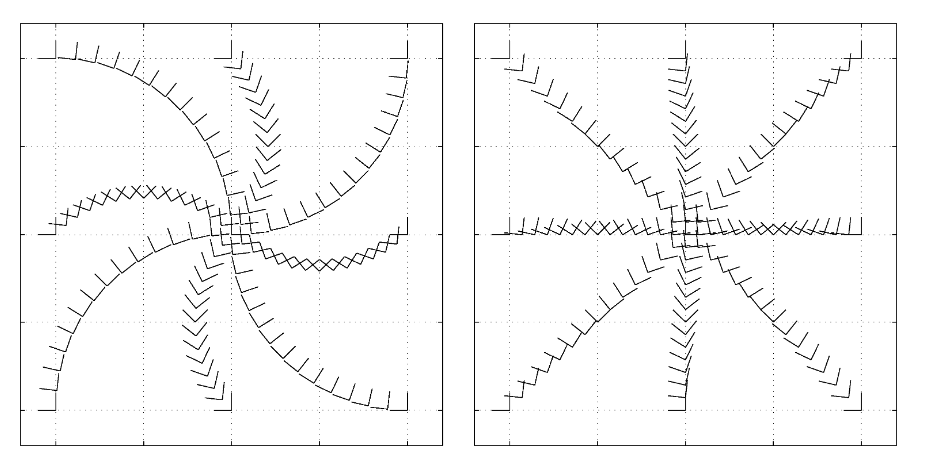
\includegraphics[width=0.90\textwidth]{figures/fig1.png}
\caption{Proportional actions on $\SE(2)$. From left to right: logarithmic function (1-parameter subgroups on $\SE(2)$) and double-geodesics for $\SO(2)\times\R^2$. Each point $g\in\SE(2)$ is depicted as a frame on the plane.}\label{fig:proportional-actions-se2}
\end{figure}

\paperremark{ (Symmetries in the control laws)}{rem:control-law-symmetries} Similar versions of the two lemmas can be easily written for the right invariant case ($\dot g=V^sg$) and some instructive behavior can be easily described. In the following, let $g_{\mathrm{left}}(t)$ and $g_{\mathrm{right}}(t)$ be the solutions to the left and right closed loop systems:
\begin{itemize}
\item To examine the logarithmic control law applied to a right invariant system, recall the basic Lie group identity $\Ad_g\log(g)=\log(g)$. Then the closed-loop systems (with unit gains),
\begin{equation*}
\dot g_{\mathrm{left}}=-g_{\mathrm{left}}\log(g_{\mathrm{left}})
\qquad\text{and}\qquad
\dot g_{\mathrm{right}}=-\log(g_{\mathrm{right}})g_{\mathrm{right}},
\end{equation*}
are the same differential equation and we have
\begin{equation*}
g_{\mathrm{left}}(0)=g_{\mathrm{right}}(0)\quad\Longrightarrow\quad
g_{\mathrm{left}}(t)=g_{\mathrm{right}}(t).\tag{4.3}\label{eq:4.3}
\end{equation*}
\item Regarding the double-geodesic control law we can state a similar but opposite result. The control law for this case is
\begin{equation*}
\begin{cases}
\omega^s=-K_\omega\rev{\Log_{\SO(3)}(R)},\\
v^s=-K_vp,
\end{cases}
\end{equation*}
and (with unit gains) the left and right closed-loop control systems are
\begin{equation*}
\begin{cases}
\dot R=-R\log_{\SO(3)}(R),\\
\dot p=-p,
\end{cases}
\qquad\text{and}\qquad
\begin{cases}
\dot R=-\log_{\SO(3)}(R)R,\\
\dot p=-\log_{\SO(3)}(R)p-p.
\end{cases}
\end{equation*}
Then easy algebraic steps show
\begin{equation*}
g_{\mathrm{left}}(0)=g_{\mathrm{right}}^{-1}(0)\quad\Longrightarrow\quad
g_{\mathrm{left}}(t)=g_{\mathrm{right}}^{-1}(t).\tag{4.4}\label{eq:4.4}
\end{equation*}
Note the peculiar correspondence between \eqref{eq:4.3} and \eqref{eq:4.4}.
\end{itemize}

\subsection{Second order systems}\label{subsec:second-order-se3}
We now apply these proportional strategies, coupled with a derivative term, to second order, fully actuated systems on $\SE(3)$. Consider the left invariant second order system
\begin{equation*}
\begin{cases}
\dot g=gV^b,\\
\dot V^b=f(g,V^b)+U,
\end{cases}\tag{4.5}\label{eq:4.5}
\end{equation*}
where $f(g,V^b),U\in\se(3)$ are internal drift and control input. The previous discussion leads to the two theorems:

\papertheorem{Regulation via the double-geodesic law}{thm:double-geodesic-regulation}{Consider the system in equation~\eqref{eq:4.5} and let $K_\omega,K_v$ and $K_d$ be the positive definite gains. Then the control law}
\begin{equation*}
U(g,V^b)=-f(g,V^b)-\begin{bmatrix}K_\omega\rev{\Log_{\SO(3)}(R)}\\R^TK_vp\end{bmatrix}-K_dV^b,\tag{4.6}\label{eq:4.6}
\end{equation*}
\emph{exponentially stabilizes the state $g$ at $I$ from any initial condition $g(0)=(R(0),p(0))$ with $\tr(R(0))\neq-1$ and for all $K_\omega$ and $\omega^b(0)$ such that}
\begin{equation*}
\lambda_{\min}(K_\omega)>\frac{\|\omega^b(0)\|^2}{\pi^2-\|R(0)\|_{\SO(3)}^2}.\tag{4.7}\label{eq:4.7}
\end{equation*}
\emph{Proof.} The scalar gain case ($K_v=K_\omega=k_p$) admits a standard proof identical to the one of Theorem~\ref{thm:pd-so3}, but with the candidate Lyapunov function
\begin{align*}
W(g,V^b)&=\frac{k_p}{2}\bigl(\|R\|_{\SO(3)}^2+\|p\|^2\bigr)+\langle V^b,V^b\rangle_{\R^6}\\
&\quad+\eps\left\langle\begin{bmatrix}\rev{\Log_{\SO(3)}(R)}\\R^Tp\end{bmatrix},V^b\right\rangle_{\R^6}.
\end{align*}
For the matrix gain case the notation becomes more involved but the algebraic steps are the same. In particular, also the sufficiency of condition~\eqref{eq:4.7} (exactly corresponding to condition~\eqref{eq:3.4}) follows from the same steps as in Theorem~\ref{thm:pd-so3}. \proofbox

\papertheorem{Regulation via the logarithm function}{thm:logarithm-regulation}{Consider the system in equation~\eqref{eq:4.5} and let $K_p$ and $K_d$ be positive-definite gains. Then the control law}
\begin{equation*}
U(g,V^b)=-f(g,V^b)-K_p\log(g)-K_dV^b,\tag{4.8}\label{eq:4.8}
\end{equation*}
\emph{locally exponentially stabilizes the state $g$ at $I\in\SE(3)$. Furthermore, if scalar gains are employed ($K_p=k_pI_6$ and $K_d=k_dI_6$), then the control law in \eqref{eq:4.8} exponentially stabilizes the state $g$ at $I$ from any initial condition $g(0)=(R(0),p(0))$ with $\tr(R(0))\neq-1$ and for all $k_p$ and $\omega^b(0)$ such that}
\begin{equation*}
k_p>\frac{\|\omega^b(0)\|^2}{\pi^2-\|R(0)\|_{\SO(3)}^2}.\tag{4.9}\label{eq:4.9}
\end{equation*}

\emph{Proof.} Given the definition of matrix logarithm on $\SE(3)$ in Lemma~\ref{lem:logarithmic-map}, the feedback law in equation~\eqref{eq:4.8} is equal up to higher order terms to the one in equation~\eqref{eq:4.6}. Thus local exponential stability is ensured.

For the scalar gains case, we can prove almost global exponential stability. Consider the closed loop system:
\begin{align*}
\dot g&=gV,\tag{4.10}\label{eq:4.10}\\
\dot V&=-k_p\log(g)-k_dV,\tag{4.11}\label{eq:4.11}
\end{align*}
starting from initial conditions $(g(0),V(0))=(g_0,V_0)\in\SE(3)\times\se(3)$. Since equation~\eqref{eq:4.11} is linear, we can decompose the solution $V$ as the sum of two components $V=V_{\mathrm{hom}}+V_{\mathrm{par}}$, where $V_{\mathrm{hom}}(t)=V_0\exp(-t/k_d)$ and $V_{\mathrm{par}}$ is the solution of \eqref{eq:4.11} with zero initial condition (and considering the $\log(g)$ term as an external disturbance).

Notice now that the manifold
\begin{equation*}
M=\{(g,V):V=\lambda\log(g),\ \text{for some }\lambda\in\R\}\subset\SE(3)\times\se(3)
\end{equation*}
is invariant for the system of ODEs \eqref{eq:4.10} and \eqref{eq:4.11} with initial conditions $(g(0),V(0))=(g_0,0)$. For, consider the system expressed in exponential coordinates
\begin{align*}
\dot X &=\rev{\JopR^{-1}(X)}V,\\ 
\dot V &=-k_pX-k_dV
\end{align*}
and substitute $X=\lambda V$ to obtain
\begin{align*}
\dot X &=\rev{\JopR^{-1}(X)}\lambda X=\lambda X,\\
\dot V &=-\frac{k_p}{\lambda}V-k_dV=-\left(\frac{k_p}{\lambda}+k_d\right)V.
\end{align*}
Hence for all $t$, $X(t)\in\operatorname{span}X(0)$ and $V(t)\in\operatorname{span}X(0)$, provided $V(0)=\lambda X(0)$. It is now easy to show that the invariant manifold $M$ is stable, since assuming $X=x\,\vers(X(0))$ and $V=v\,\vers(X(0))$ we have
\begin{equation*}
\dot x=v,\qquad \dot v=-k_px-k_dv\quad\Longrightarrow\quad \ddot x=-k_px-k_d\dot x.\tag{4.12}\label{eq:4.12}
\end{equation*}
The proof is now complete by noting that the original system \eqref{eq:4.10} and \eqref{eq:4.11} can be written as
\begin{equation*}
\dot X=\rev{\JopR^{-1}(X)}V=\rev{\JopR^{-1}(X)}V_{\mathrm{par}}+\rev{\JopR^{-1}(X)}V_{\mathrm{hom}},
\end{equation*}
\begin{equation*}
\dot V=-k_pX-k_dV=-k_pX-k_dV_{\mathrm{par}}-k_dV_{\mathrm{hom}},
\end{equation*}
where the disturbance$
\begin{bmatrix}\rev{\JopR^{-1}(X)}V_{\mathrm{hom}}\\-k_dV_{\mathrm{hom}}\end{bmatrix}
$
decreases to zero exponentially. Lemma~\ref{lem:se3-exp-coordinate-derivative}.7 in Khalil \cite{18} applies proving local exponential stability.

Additionally, if condition~\eqref{eq:4.9} is satisfied, then with the same bounding technique in the proof of Theorem~\ref{thm:pd-so3}, we can prove that no singularity will be encountered by the closed loop trajectories. \proofbox

\paperremark{}{rem:right-invariant-se3} As usual we can extend to the right invariant case ($\dot g=V^sg$) all we have done for the left one. For both systems the logarithmic control law (in Theorem~\ref{thm:logarithm-regulation}) is identical. The double-geodesic law applied to a right system has the slightly different expression:
\begin{equation*}
U(g,V^s)=-f(g,V^s)-\begin{bmatrix}K_\omega\rev{\Log_{\SO(3)}(R)}\\K_vp\end{bmatrix}-K_dV^s.
\end{equation*}

\paperexample{ (Workspace control of mechanical systems)}{ex:workspace-control} As in Example~\ref{ex:satellite-orientation} for $\SO(3)$, we here apply our control strategies to fully actuated mechanical systems. Examples of this class of systems are robotic manipulators and 6 degree of freedom (DOF) underwater vehicles. We assume here that a change of coordinates and inputs has already been applied to the system so that our model is described by
\begin{equation*}
\begin{cases}
\dot g=gV^b,\\
M(g)\dot V^b=-C(g,V^b)V^b-N(g,V^b)+U,
\end{cases}
\end{equation*}
where $M(g)$ is the inertia matrix, $C(g,V^b)$ is the Coriolis matrix and $N(g,V^b)$ is used to model friction and gravity. The kinetic energy of this mechanical system is computed with the positive definite form \eqref{eq:4.1} (coupled with the left translation of the velocity $gV^b$). Hence, for this class of systems, we are naturally led to prefer the double-geodesic control law over the logarithmic one:
\begin{equation*}
U(g,V^b)=N(g,V^b)-\begin{bmatrix}k_\omega\rev{\Log_{\SO(3)}(R)}\\k_vR^Tp\end{bmatrix}-K_dV^b.\tag{4.13}\label{eq:4.13}
\end{equation*}
Exponential stability is proved through the Lyapunov function
\begin{align*}
W(g,V^b)&=\frac{k_\omega}{2}\|R\|_{\SO(3)}^2+\frac{k_v}{2}\|p\|^2+\langle V^b,M(g)V^b\rangle_{\R^6}\\
&\quad+\eps\left\langle\begin{bmatrix}\rev{\Log_{\SO(3)}(R)}\\R^Tp\end{bmatrix},M(g)V^b\right\rangle_{\R^6}.
\end{align*}
Once again, in writing equation~\eqref{eq:4.13} we take advantage of the passivity properties of the Coriolis term $C(g,V^b)V^b$ and we compensate only for $N(g,V^b)$. Rather than canceling both terms, this approach appears to be a more natural way of controlling fully actuated mechanical systems, see Koditschek's early work \cite{19} for more details.

A few remarks:
\begin{enumerate}
\item The control law in equation~\eqref{eq:4.13} has the usual advantages of PD control described in \cite{26}: ease of computation and no knowledge of the exact system's parameters required.
\item A second approach would involve a typical ``computed torque'' technique, where the Coriolis term $C$ is explicitly compensated for. In this latter case, the logarithmic control law of Theorem~\ref{thm:logarithm-regulation} can be applied.
\end{enumerate}
Future avenues of research consists in the application of the logarithmic control law for the case of robotic manipulators for the purpose of hybrid (position/force) control and the study from a (Lie group) algebraic viewpoint if simplifications occur in the expression of the Jacobian manipulator (again, when logarithmic control law is applied).

\paperexample{ (Position and attitude stabilization of planar rigid body)}{ex:planar-stabilization} To compare the two classes of controllers presented above, we consider the problem of stabilizing a planar rigid body. Note that the subgroup of the planar motions $\SE(2)$ contains still most of the complexity and richness of the full $\SE(3)$ case.

We have simulated the feedback laws described in Theorem~\ref{thm:double-geodesic-regulation} and~\ref{thm:logarithm-regulation} (double-geodesic and logarithmic laws for left invariant systems), and in Remark~\ref{rem:right-invariant-se3} (double-geodesic and logarithmic law for right systems). As foreseen from theoretical considerations, the logarithmic control law generates the same closed-loop trajectories for both the right and the left invariant systems. The shape of the trajectories for all of the cases varies considerably depending on the size of the initial angle error and on the gain values: for all cases we picked an initial rotational error equal to $\pi/2$ and we choose two sets of scalar gains: $(k_p,k_d)=(1,2)$ and $(k_p,k_d)=(1,1)$. We here report the $\SE(2)$ trajectories for the 4 controllers with the first set of gains (Figures~\ref{fig:left-invariant-trajectories} and~\ref{fig:right-invariant-trajectories}) and the corresponding velocity profiles for the two left invariant controllers, (Figures~\ref{fig:velocity-double-geodesic} and~\ref{fig:velocity-logarithmic}). Also we show in Figure~\ref{fig:low-derivative-gain} how the trajectories change when a low derivative gain $k_d$ is applied (low with respect to a constant proportional gain).

Looking at the plots in Figure~\ref{fig:left-invariant-trajectories} and 3 a few simple remarks can be made:
\begin{enumerate}
\item In agreement with the fact that the various feedbacks are equal in the rotational part, the angular behavior is the same in all simulations.
\item All the control laws seem to converge at a very similar rate in both the rotational (of course) and translational part. This is also predictable since identical gains are applied. Indeed, quantitative results (which we don't report for brevity) indicate that the various input norms for the logarithmic control law are larger than for the double-geodesic strategy. Typically the logarithmic inputs would be about 10\% larger than the double geodesics (see Figure~\ref{fig:velocity-double-geodesic} and~\ref{fig:velocity-logarithmic}).
\item Qualitatively, the clearest difference regards the opposite handedness of the various control laws. Corresponding to a choice of left invariant control system the logarithmic and double-geodesic feedbacks will follow quite different paths even from a simple qualitative viewpoint (Figure~\ref{fig:left-invariant-trajectories}). In the right invariant case instead the handedness is the same, but the double-geodesic law shows a more curved behavior (Figure~\ref{fig:right-invariant-trajectories}).
\item The difference in the shape of trajectories becomes even clearer in second simulation in Figure~\ref{fig:low-derivative-gain} where a low derivative gain $k_d$ is employed and where the effects of the different proportional actions is therefore emphasized. Note the oscillatory behaviour of both closed loop system: the values $(k_p,k_d)=(1,1)$ corresponds to an slightly damped second order systems. This kind of behaviour seems therefore maintained by our nonlinear models.
\end{enumerate}
The issues described in Remark~\ref{rem:control-law-symmetries} on symmetries of control laws and the proof of Theorem~\ref{thm:logarithm-regulation}, find clear illustration in the case of high derivative gain (first set of simulations). Notice that:
\begin{enumerate}[resume]
\item both left and right invariant closed loop systems with logarithmic control law remain on the 1-parameter subgroup of $\SE(3)$ determined by the initial conditions (see right pictures in Figure~\ref{fig:left-invariant-trajectories} and~\ref{fig:low-derivative-gain}). In Figure~\ref{fig:velocity-double-geodesic} and~\ref{fig:velocity-logarithmic} we report the time evolution of the velocity $V=(v_x,v_y)$. In the logarithmic control case, since the state remains on a 1-parameter subgroup, the ratio of the inputs $v_x/v_y$ remains constant during the simulation, see Figure~\ref{fig:velocity-logarithmic} compared to Figure~\ref{fig:velocity-double-geodesic}. These facts are predicted and are at the basis of the proof of Theorem~\ref{thm:logarithm-regulation}.
\item modulo the differing initial conditions, we recover the trajectories of the left double-geodesic closed loop system by inverting the right double-geodesic trajectories.
\end{enumerate}

\begin{figure}[htbp]
\centering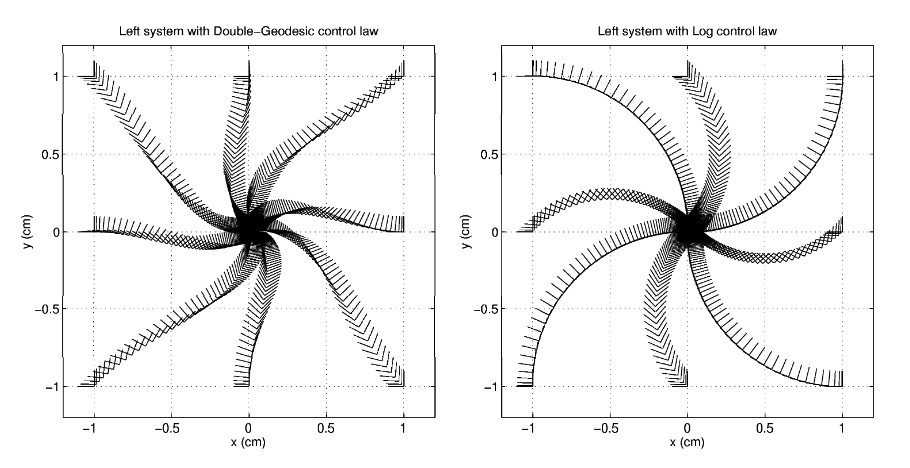
\includegraphics[width=0.90\textwidth]{figures/fig2.png}
\caption{Trajectories of left invariant control systems on $\SE(2)$. From left to right: double-geodesic control law as in Theorem~\ref{thm:double-geodesic-regulation} and logarithmic control law as in Theorem~\ref{thm:logarithm-regulation}. Each point $g\in\SE(2)$ is depicted as a frame on the plane. Note the opposite handedness of the two control strategies.}\label{fig:left-invariant-trajectories}
\end{figure}
\begin{figure}[htbp]
\centering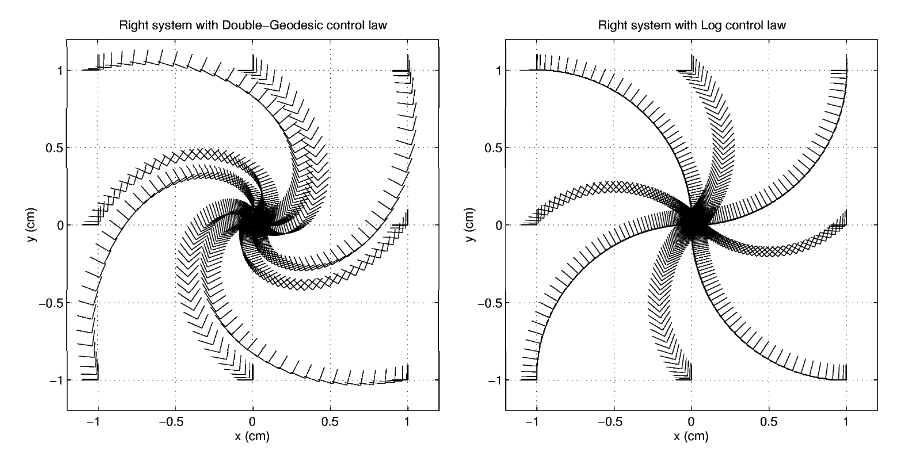
\includegraphics[width=0.90\textwidth]{figures/fig3.png}
\caption{Trajectories of right invariant control systems on $\SE(2)$. From left to right: double-geodesic control law as in Remark~\ref{rem:right-invariant-se3} and logarithmic control law as in Theorem~\ref{thm:logarithm-regulation}.}\label{fig:right-invariant-trajectories}
\end{figure}
\begin{figure}[htbp]
\centering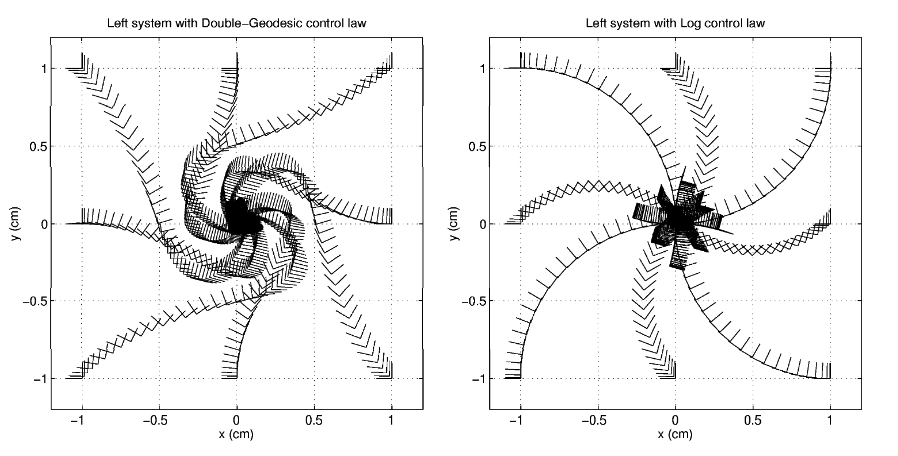
\includegraphics[width=0.90\textwidth]{figures/fig4.png}
\caption{Trajectories of left invariant control systems on $\SE(2)$ with low derivative gain $k_d$. From left to right: double-geodesic control law as in Theorem~\ref{thm:double-geodesic-regulation} and logarithmic control law as in Theorem~\ref{thm:logarithm-regulation}. Note that the state of the closed loop system with logarithmic control law (on the right) remains on the 1-parameter subgroup determined by the initial condition. The double-geodesic control law instead gives rise to a spiraling $(x,y)$ motion (on the left).}\label{fig:low-derivative-gain}
\end{figure}
\begin{figure}[htbp]
\centering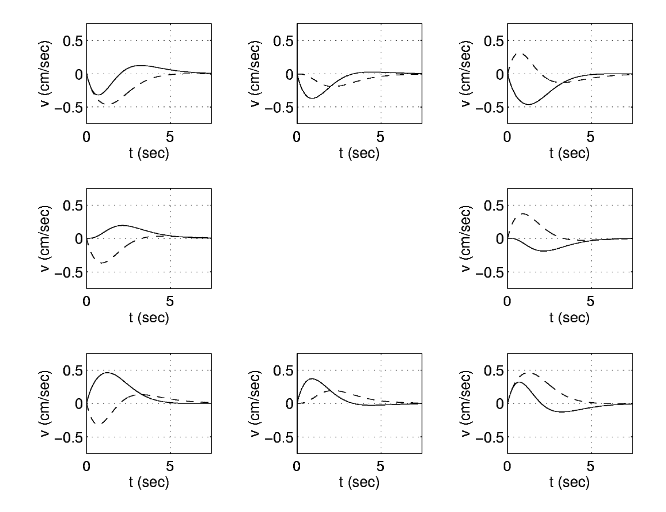
\includegraphics[width=0.70\textwidth]{figures/fig5.png}
\caption{Velocity profiles of double-geodesic control law for the simulation depicted in Figure~\ref{fig:left-invariant-trajectories}. The eight figures show the time evolution of $v_x(t),v_y(t)$ from the eight initial conditions: the location of the 8 pictures corresponds to the 8 initial condition in the $(x,y)$ plane.}\label{fig:velocity-double-geodesic}
\end{figure}
\begin{figure}[htbp]
\centering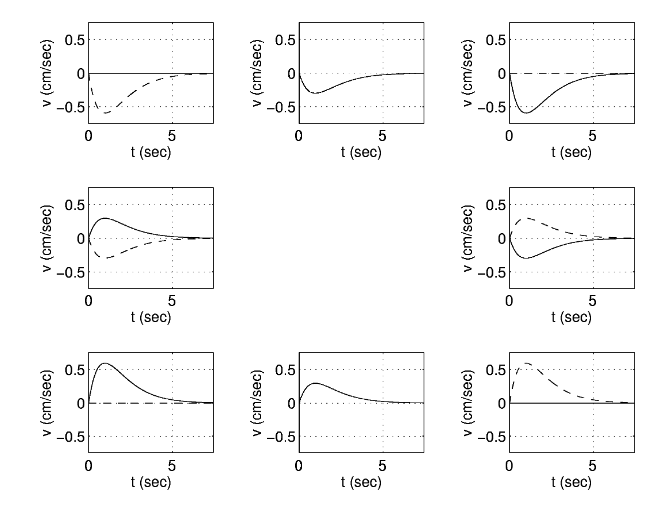
\includegraphics[width=0.70\textwidth]{figures/fig6.png}
\caption{Same as above, but for the logarithmic control law. Note that the input magnitude is slightly larger for logarithmic rather than for double-geodesic control law. Also, in the logarithmic case, the ratio $v_x/v_y$ is constant for all initial conditions, since the state $g\in\SE(2)$ remains on the 1-parameter subgroup $\exp(\lambda\log(g(0)))$ for all time.}\label{fig:velocity-logarithmic}
\end{figure}

\section{Trajectory tracking}\label{sec:trajectory-tracking}
We describe here a general approach to trajectory tracking problems for second order systems defined on Lie groups. In particular, by exploiting the group structure we reduce the tracking problem to a stabilization one for an appropriately defined error system.

In the following, we will assume that we are given a left invariant, second order control system on $G$
\begin{equation*}
\begin{cases}
\dot g=gV,\\
\dot V=f(g,V)+U,
\end{cases}\tag{5.1}\label{eq:5.1}
\end{equation*}
and a control law $U=Z(g,V)$ that makes the closed loop driftless system $\dot g=gV$, $\dot V=Z(g,V)$ locally asymptotically (exponentially) stable at the identity $e_G=I$. We want to design a control law that makes the state $g$ track a reference trajectory $g_d\in G$ described by: $\dot g_d=V_dg_d$, for $V_d(t)\in\gfrak$.

\subsection{Choices of error function on $\SE(3)$}\label{subsec:error-functions-se3}
In order to define a correct notion of error function, we exploit the natural group structure of the configuration manifold, see for example \cite{34}.

Given the interpretation of group elements on $\SE(3)$ as coordinate frames, the natural choice of state error is
\begin{equation*}
e\triangleq g_d^{-1}g,
\end{equation*}
which represents the reference frame as ``seen'' from the state of the system. In other words, if $g$ represents the body frame and $g_d$ the desired frame, then $e$ is the relative $g$ to $g_d$ frame. Decomposing this error in its rotational and translational components, we have:
\begin{equation*}
e=\begin{bmatrix}R_d^TR&R_d^T(p-p_d)\\0&1\end{bmatrix}.\tag{5.2}\label{eq:5.2}
\end{equation*}
We call this the \emph{natural error}. An equivalent definition would be $g^{-1}g_d\equiv e^{-1}$, since, as described in Section~\ref{sec:pd-se3}, controlling $e$ or $e^{-1}$ is the same control problem.

If we discard the physical reasoning associated with the natural definition, other choices of configuration error are possible. In particular the following two appear appealing:
\begin{enumerate}
\item Define the \emph{reciprocal error} as
\begin{equation*}
e_{\mathrm{recip}}\triangleq gg_d^{-1}=\begin{bmatrix}RR_d^T&p-RR_d^Tp_d\\0&1\end{bmatrix},\tag{5.3}\label{eq:5.3}
\end{equation*}
where we exchange the order of multiplication.
\item In keeping with the notation in \cite{26}, define the \emph{hybrid error} as
\begin{equation*}
e_{\mathrm{hybrid}}\triangleq\begin{bmatrix}R_d^TR&p-p_d\\0&1\end{bmatrix},\tag{5.4}\label{eq:5.4}
\end{equation*}
where we keep the natural error choice for the rotational part (we could instead have $RR_d^T$).
\end{enumerate}

Even though these latter two definitions seem also rather natural, the Lie group structure of the original problem is not taken into account. It happens in particular that reciprocal and hybrid error (between body and desired frame) depend on the arbitrary choice of inertial frame. For, recall that a change of inertial frame corresponds to a left translation. Thus consider the map $L_{g_0}$ such that $L_{g_0}g=g_0g$ and $L_{g_0}g_d=g_0g_d$. Then, if $g_0=(R_0,p_0)$, we have
\begin{equation*}
e'_{\mathrm{recip}}=\begin{bmatrix}R_0RR_d^TR_0^T&p-R_0RR_d^TR_0^Tp_d\\0&1\end{bmatrix},
\end{equation*}
\begin{equation*}
e'_{\mathrm{hybrid}}=\begin{bmatrix}R^TR_d&R_0(p-p_d)\\0&1\end{bmatrix}.
\end{equation*}
Note that for the hybrid error, this inertial frame dependency simply implies the presence of an arbitrary rotation in the translational part. For the reciprocal error instead, more evident effects appear: for example, even for $p=p_d$, i.e. for overlapping frames, $e_{\mathrm{recip}}$ ``sees'' some translational error if $R\neq R_d$. This will reflect in a control law with non-zero translational input, which is undoubtedly undesired.

Eventually note that the drawbacks just described affect also the inverse definitions $e_{\mathrm{recip}}^{-1}$ and $e_{\mathrm{hybrid}}^{-1}$. Therefore, after this theoretical discussion, we tend to prefer the natural choice \eqref{eq:5.2}; the simulations performed later will further clarify the final choice.

\subsection{Basic properties of dynamical systems on Lie groups}\label{subsec:dynamics-lie-groups}
We characterize here the behavior of the composition of systems defined on the group $G$. Recall that, given $l,r\in G$ and $L,R\in\gfrak$, we call $\dot l=lL$ a \emph{left control system} and $\dot r=Rr$ a \emph{right control system}. Also, given two systems with state $g(t),h(t)\in G$, we call the \emph{inverse system} the one corresponding to the state $g(t)^{-1}$ and the \emph{product system} the one corresponding to the state $g(t)h(t)$.

By performing some chain rule differentiations, we have:

\paperlemma{Time derivative of composed systems}{lem:composed-systems}{With the notation just introduced it holds}
\begin{equation*}
\dot l^{-1}=-Ll^{-1},\qquad \dot r^{-1}=-r^{-1}R,
\end{equation*}
\emph{and}
\begin{equation*}
(gh)^{-1}\frac{d(gh)}{dt}=\Ad_{h^{-1}}(g^{-1}\dot g)+h^{-1}\dot h,
\end{equation*}
\begin{equation*}
\frac{d(gh)}{dt}(gh)^{-1}=\dot gg^{-1}+\Ad_g(\dot hh^{-1}),
\end{equation*}
\emph{where the adjoint map $\Ad$ is defined in Section~\ref{sec:systems-lie-groups}.}

By means of these basic results, we are able to describe straightforwardly how, for instance, the product of two left control systems evolves in time: letting $\dot l_1=l_1L_1$ and $\dot l_2=l_2L_2$, we have
\begin{equation*}
\frac{d}{dt}l_1l_2=l_1l_2(\Ad_{l_2^{-1}}L_1+L_2).\tag{5.5}\label{eq:5.5}
\end{equation*}

\paperlemma{Derivative of adjoint map}{lem:adjoint-derivative}{Let $U(t)\in\gfrak$, $\dot l=lL$ and $\dot r=Rr$, with $l,r\in G$ and $L,R\in\gfrak$. Then}
\begin{align*}
\frac{d}{dt}\bigl(\Ad_{l(t)}U(t)\bigr)&=\Ad_l\dot U+\Ad_l[L,U],\\
\frac{d}{dt}\bigl(\Ad_{r(t)}U(t)\bigr)&=\Ad_r\dot U+[R,\Ad_rU].
\end{align*}
Now, recalling equation~\eqref{eq:5.5}, we can define $l_{12}\triangleq l_1l_2$ and $V_{12}\triangleq\Ad_{l_2^{-1}}L_1+L_2$. Lemma~\ref{lem:adjoint-derivative} gives:
\begin{equation*}
\begin{cases}
\dot l_{12}=l_{12}V_{12},\\
\dot V_{12}=\Ad_{l_2^{-1}}\dot L_1+[\Ad_{l_2^{-1}}L_1,L_2]+\dot L_2,
\end{cases}\tag{5.6}\label{eq:5.6}
\end{equation*}
which shows how we can write in full generality the second order dynamics of the combination of Lie group systems.

\subsection{Extending regulators to trajectory trackers}\label{subsec:regulators-to-trackers}
We are now able to formulate the following general solution:

\papertheorem{Trajectory tracking}{thm:trajectory-tracking}{Consider the system in equation~\eqref{eq:5.1}, the asymptotic (exponential) regulator law $Z(g,V)$ and the desired trajectory $g_d(t)$. Define the configuration error $e\triangleq g_d^{-1}g\in G$ and the velocity error $V_e\triangleq V-\Ad_{g^{-1}}V_d\in\gfrak$. Then the control law}
\begin{equation*}
U=U_{\mathrm{ff}}(g,V)+U_{\mathrm{tr}}(g,V,V_d,\dot V_d)+Z(e,V_e)\tag{5.7}\label{eq:5.7}
\end{equation*}
\emph{where}
\begin{equation*}
U_{\mathrm{ff}}(g,V)=-f(g,V),
\end{equation*}
\begin{equation*}
U_{\mathrm{tr}}(g,V,V_d,\dot V_d)=\Ad_{g^{-1}}(\dot V_d)+[\Ad_{g^{-1}}(V_d),V],
\end{equation*}
\emph{makes the configuration error $e$ locally asymptotically (exponentially) approach the identity $I\in G$.}

\emph{Proof.} The result follows straightforwardly from equation~\eqref{eq:5.6}. Indeed consider the error $e=g_d^{-1}g$ and its velocity $V_e=V-\Ad_{g^{-1}}V_d$. Then the addenda in equation~\eqref{eq:5.7} cancel out exactly the extra pieces in equation~\eqref{eq:5.6} and the closed loop system satisfies
\begin{equation*}
\dot V_e=Z(e,V_e).
\end{equation*}
By assumption, asymptotic (exponential) stability is proven. \proofbox

A few comments: first, for the $\SO(3)$ case we can simplify the tracking law by defining $U_{\mathrm{tr}}=\Ad_{g^{-1}}\dot V_d$. The PD control law in equation~\eqref{eq:3.3} would still ensure exponential stability thanks to the orthogonality properties discussed in Subsection~\ref{subsec:metric-compact}.

Second, in stating Theorem~\ref{thm:trajectory-tracking}, we assumed our control system to be left invariant and our trajectory to be right invariant. These two choices are suited to the kind of mechanical systems we are interested in, such as example satellite reorienting and robotic manipulation. However, similar versions of the theorem can be stated using any combination of right and left invariant systems.

Eventually, Theorem~\ref{thm:trajectory-tracking} can be stated for the other definitions of error function: reciprocal and hybrid.
\begin{enumerate}
\item For the case of $e_{\mathrm{recip}}$, the results obtained in the previous subsection lead straightforwardly to
\begin{equation*}
\begin{cases}
\dot e_{\mathrm{recip}}=e_{\mathrm{recip}}(\Ad_{g_d}V-V_d)\triangleq e_{\mathrm{recip}}V_e,\\
\dot V_e=\Ad_{g_d}(f(g,V)+U)-\dot V_d+[V_d,\Ad_{g_d}V],
\end{cases}
\end{equation*}
and similarly to equation~\eqref{eq:5.7} we set
\begin{equation*}
U=\Ad_{g_d^{-1}}\bigl(U_{\mathrm{ff}}+U_{\mathrm{tr}}+Z(e_{\mathrm{recip}},V_e)\bigr),
\end{equation*}
where $U_{\mathrm{tr}}=\dot V_d-[V_d,\Ad_{g_d}V]$ and $U_{\mathrm{ff}}=-f(g,V)$.
\item For the hybrid error instead, we want to keep the computations in local coordinates $(R,p)$: from definition \eqref{eq:5.4} we have $p_e\triangleq p-p_d$ and $R_e=R_d^TR$. For the rotational part $R_e\in\SO(3)$, we apply Theorem~\ref{thm:trajectory-tracking}; for the translational part we have
\begin{equation*}
\dot p_e=Rv-v_d,
\end{equation*}
\begin{equation*}
\ddot p_e=R(f_t(g,V)+a)-\dot v_d+R(\omega\times v),
\end{equation*}
where $a\in\R^3$ is the acceleration input and $f_t$ is the drift in the translational coordinates (see equation~\eqref{eq:5.1}). So we can write $U=(\tau,a)$, where $\tau$ is chosen from the previous theorem and a PD controller for the translation part gives
\begin{equation*}
a=a_{\mathrm{ff}}+a_{\mathrm{tr}}+R^T(-k_pp_e-k_d\dot p_e),\tag{5.8}\label{eq:5.8}
\end{equation*}
where $a_{\mathrm{tr}}=v\times\omega$ and $a_{\mathrm{ff}}=-f_t(g,V)$.
\end{enumerate}

\paperexample{ (Position and attitude tracking on $\SE(2)$)}{ex:se2-tracking} To compare the various error choice presented above, we consider the trajectory tracking problem for a planar rigid body. This control problem models for example a robot manipulator spray painting planar objects.

We have simulated the trajectory tracking strategies just described for the second order system \eqref{eq:5.1} with no internal drift: $f(g,V)=0$. To recall the notation, our system is
\begin{equation*}
\begin{bmatrix}\dot\theta\\\dot x\\\dot y\end{bmatrix}
=\begin{bmatrix}1&0&0\\0&\cos\theta&-\sin\theta\\0&\sin\theta&\cos\theta\end{bmatrix}
\begin{bmatrix}\omega\\v_x\\v_y\end{bmatrix},
\qquad
\begin{bmatrix}\dot\omega\\\dot v_x\\\dot v_y\end{bmatrix}=U.
\end{equation*}
The reference trajectory has the shape of an L character in the $(x,y)$ variables and it specifies the reference angle $\theta$ to be parallel to the normal vector of the planar curve. Thus the reference trajectory is discontinuous in $\theta(t)$ and in the linear velocities $v_x(t)$ and $v_y(t)$. To explicitly show the differences due to the various error choices, we intentionally run the simulations without including the additional term $U_{\mathrm{tr}}$ (no $U_{\mathrm{ff}}$ is necessary since the system we simulate is driftless). Indeed, assuming proportional and derivative gains are high enough, a simple PD control without feedforward does the job nicely; we picked $(k_p,k_d)=(3,6)$.

Recalling the PD approach in equation~\eqref{eq:5.8} for the hybrid error case, for natural and reciprocal error functions we employed the double-geodesic control law as the $Z$ regulator in Theorem~\ref{thm:trajectory-tracking}.

We report in Figure~\ref{fig:tracking-natural-hybrid} and 8 the time evolution of the state $g=(\theta,x,y)\in\SE(2)$ depicted as a straight line on the plane. In the first figure we report the natural and hybrid error cases, while in the second Figure we show the reciprocal error without and with left translation by $g_0=(\pi/2,1,1)$. The simulations start from the upper left corner of the L character and run clockwise: the linear velocity of the reference path is constant and equal to 1 cm/sec, the angular velocity is always equal to zero (but the angle evolution has steps at each corner).

A few conclusions can be easily drawn:
\begin{enumerate}
\item Theorem~\ref{thm:trajectory-tracking} with natural error function and double-geodesic regulator is exactly equivalent to hybrid error function and double-geodesic approach described in equation~\eqref{eq:5.8}. It turns out therefore that, even though the hybrid error definition is inertial frame dependent, this dependence disappears in the closed loop (the correct simplifications take place).
\item The reciprocal error function (coupled with the approach in Theorem~\ref{thm:trajectory-tracking} and a double-geodesic regulator) shows both the drawbacks discussed in Subsection~\ref{subsec:error-functions-se3}: an error in the rotational part affects the translational part and an inertial frame translation changes the closed loop trajectories (compare left to right picture in Figure~\ref{fig:tracking-reciprocal}).
\end{enumerate}
We eventually draw some conclusions: the theoretical analysis in the previous subsections and the numerical simulations here presented, suggest that the natural error function defined in equation~\eqref{eq:5.2} is the correct choice. While the reciprocal error function shows some evident drawbacks, the hybrid error in equation~\eqref{eq:5.4} (coupled with the strategy described in the previous subsection) represents an equivalent choice. Nevertheless the definition of hybrid error on $\SE(3)$ relies on the natural error function for the rotational part and needs a distinct control design (it is not possible to extend point stabilizers into trajectory trackers in a straightforward manner).

\begin{figure}[htbp]
\centering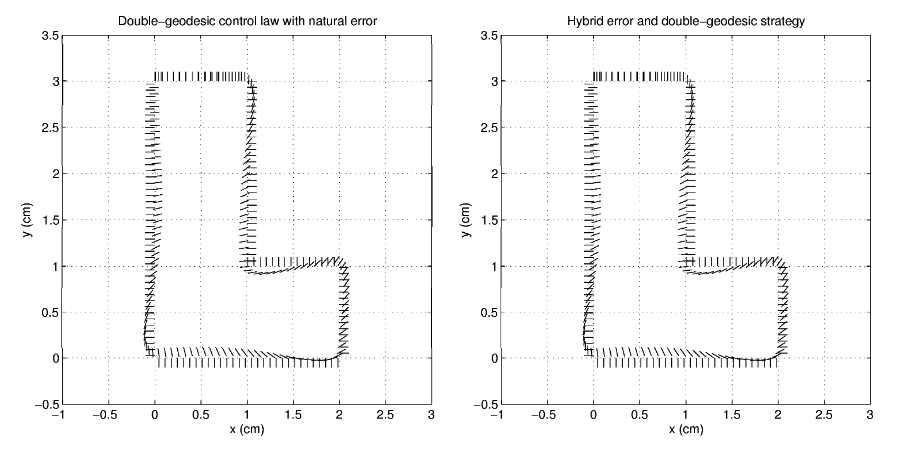
\includegraphics[width=0.90\textwidth]{figures/fig7.png}
\caption{Trajectory tracking for left invariant second order systems. On the left natural error, on the right hybrid error: they are identical pictures. As the pictures confirm, it is equivalent to apply a double-geodesic strategy in Theorem~\ref{thm:trajectory-tracking} with the natural error function or to use the hybrid error definition and then use a double-geodesic strategy in local coordinates \eqref{eq:5.8}.}\label{fig:tracking-natural-hybrid}
\end{figure}
\begin{figure}[htbp]
\centering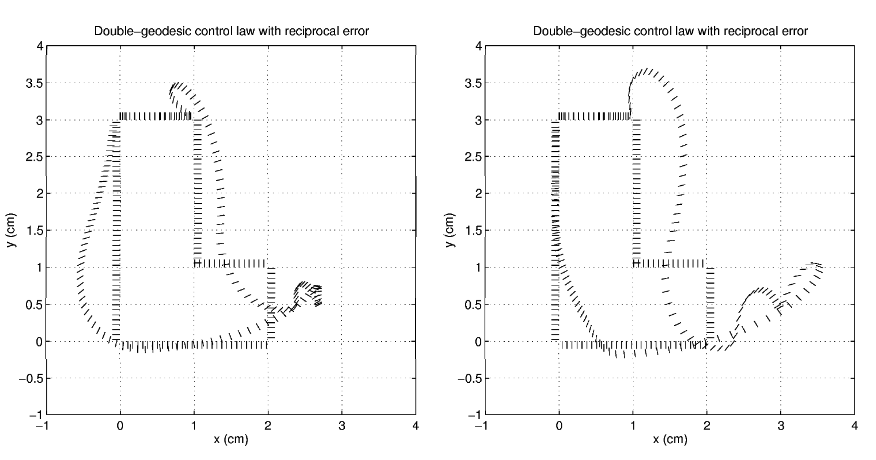
\includegraphics[width=0.90\textwidth]{figures/fig8.png}
\caption{Trajectory tracking with Theorem~\ref{thm:trajectory-tracking} applied with reciprocal error function. The simulation on the right shows the dependence of the scheme on an arbitrary left translation. As described in Subsection~\ref{subsec:error-functions-se3}, errors in the rotational part affect the translational part.}\label{fig:tracking-reciprocal}
\end{figure}

\section{Linear and homogeneous approximations of systems on the Euclidean group}\label{sec:linear-homogeneous}
So far we have focused our attention on fully actuated control systems, where the number of independent control inputs is equal to number of position variables (and in our case to the dimension of the group). More challenging control problems arise when dealing with underactuated mechanical systems possibly defined on manifolds of the form $G\times M$. A classic example of a purely Lie group system is the underactuated satellite model, which can be described as
\begin{equation*}
\dot g=g(\widehat\xi_1u_1+\cdots+\widehat\xi_mu_m),
\end{equation*}
with $\widehat\xi_i\in\gfrak$ and $m<\dim(G)$. More generally many interesting locomotion systems have also internal ``shape'' variables. For example the model of a car with two trailers falls into this class and can be written as
\begin{align*}
\dot g &=g\begin{bmatrix}1\\0\\\dfrac{1}{L_2}\tan(r_2)\end{bmatrix}^{\!\wedge}v, \\
\dot r_2 &=\left[\frac1{L_1}\frac{\tan(r_1)}{\cos(r_2)}-\frac1{L_2}\tan(r_2)\right]v,\\
\dot r_1 &=\omega,
\end{align*}
where $g\in\SE(2)$ and the operator $\widehat{\phantom{x}}$ maps $\R^3$ to $\se(2)$ in the standard way. We now concentrate on a toy example and show how to generalize some of the techniques introduced so far.

\subsection{Motivating example}\label{subsec:motivating-example}
Following \cite{32} and \cite{27}, we write a simplified kinematic model for aircrafts and underwater vehicles on $\SE(3)$ as
\begin{equation*}
\dot g=g\begin{bmatrix}
0&-\omega_3&\omega_2&v\\
\omega_3&0&-\omega_1&0\\
-\omega_2&\omega_1&0&0\\
0&0&0&0
\end{bmatrix},
\end{equation*}
where we assume we only have 4 independent actuators: velocity along the $x$ axis and the three angular velocities. We want to globally track a reference trajectory $\dot g_d=g_dV_d$, where $V_d$ lies in the subspace of feasible velocities.

Define the error attitude as $R_e=R_d^TR$ and the error position as $z_e=R^T(p-p_d)$ (see later for an interpretation). Then, with some easy algebra, we write the error equations as
\begin{equation*}
\dot R_e=R_e\widehat\omega_e,
\end{equation*}
\begin{equation*}
\dot z_e=z_e\times\omega+\begin{bmatrix}v\\0\\0\end{bmatrix}-R_e^T\begin{bmatrix}v_d\\0\\0\end{bmatrix},\tag{6.1}\label{eq:6.1}
\end{equation*}
where $\omega_e=\omega-R_e^T\omega_d$.

\paperlemma{An asymptotically stable tracking feedback}{lem:tracking-feedback}{Given the system \eqref{eq:6.1}, let $z_{e1}$ be the first component of $z_e$ and $\widehat\psi_e=\log(R_e)$. Then the control law}
\begin{equation*}
v=v_d-k_1z_{e1},\tag{6.2}\label{eq:6.2}
\end{equation*}
\begin{equation*}
\omega=R_e^T\omega_d-k_2\psi_e+
\left(\frac{\sin\|\psi_e\|}{\|\psi_e\|}\widehat z_e-\frac{1-\cos\|\psi_e\|}{\|\psi_e\|^2}\widehat z_e\widehat\psi_e\right)
\begin{bmatrix}v_d\\0\\0\end{bmatrix}\tag{6.3}\label{eq:6.3}
\end{equation*}
\emph{ensures global asymptotic stability as long as $v_d\neq0$.}

\emph{Proof.} Consider the candidate Lyapunov function
\begin{equation*}
W(R_e,z_e)=\frac12\|R_e\|_{\SO(3)}^2+\frac12\|z_e\|^2,
\end{equation*}
and differentiate with respect to time
\begin{equation*}
\frac{d}{dt}W=\langle\psi_e,\omega_e\rangle+
\left\langle z_e,\begin{bmatrix}v\\0\\0\end{bmatrix}-R_e^T\begin{bmatrix}v_d\\0\\0\end{bmatrix}\right\rangle,
\end{equation*}
where we exploit as usual the properties of exponential coordinates. Substituting \eqref{eq:6.2} we have
\begin{equation*}
\frac{d}{dt}W=-k_1z_{e1}^2+\langle\psi_e,\omega_e\rangle+
\left\langle z_e,(I-R_e^T)\begin{bmatrix}v_d\\0\\0\end{bmatrix}\right\rangle
\end{equation*}
and plugging in Rodrigues' formula from Lemma~\ref{lem:exponential-map}
\begin{align*}
\frac{d}{dt}W&=-k_1z_{e1}^2+\langle\psi_e,\omega_e\rangle+
\left\langle z_e,\widehat\psi_e\left(\frac{\sin\|\psi_e\|}{\|\psi_e\|}I-\frac{1-\cos\|\psi_e\|}{\|\psi_e\|^2}\widehat\psi_e\right)\begin{bmatrix}v_d\\0\\0\end{bmatrix}\right\rangle\\
&=-k_1z_{e1}^2+\langle\psi_e,\omega_e\rangle-
\left\langle\psi_e,\widehat z_e\left(\frac{\sin\|\psi_e\|}{\|\psi_e\|}I-\frac{1-\cos\|\psi_e\|}{\|\psi_e\|^2}\widehat\psi_e\right)\begin{bmatrix}v_d\\0\\0\end{bmatrix}\right\rangle.
\end{align*}
The control law in equation~\eqref{eq:6.3} cancels out exactly the last addend and gives
\begin{equation*}
\frac{d}{dt}W=-k_1z_{e1}^2-k_2\|\psi_e\|^2=-k_1z_{e1}^2-k_2\|R_e\|_{\SO(3)}^2,\tag{6.4}\label{eq:6.4}
\end{equation*}
proving the Lyapunov stability of the closed-loop system.

We can now invoke Lasalle's principle to prove asymptotic stability: the closed-loop trajectories of the system converge asymptotically to the largest invariant set contained in
\begin{equation*}
\Omega\{(R_e,z_e):\dot W=0\}=\{(R_e,z_e)\in\SE(3):R_e=I\text{ and }z_{e1}=0\},
\end{equation*}
and since in $\Omega$ the dynamic equation of the closed-loop system reduces to
\begin{equation*}
0=\omega_e=\widehat z_e\begin{bmatrix}v_d\\0\\0\end{bmatrix},
\end{equation*}
then, as long as $v_d\neq0$, the largest invariant set contained in $\Omega$ is the set $\{(I,0)\}$. \proofbox

Despite the successful analysis for this toy example, the kind of technique we have pursued so far cannot be generalized to solve generic point stabilization problems and tracking problems for second order driftless systems or underactuated systems with drift (for example). For these cases various approaches have been developed in the literature. Here we restrict our interest to the following issues:
\begin{enumerate}
\item \emph{Jacobian linearization for gain scheduling design.} For this standard approach to trajectory tracking we here derive simplified Jacobian linearizations of systems defined on $\SO(3)$ and $\SE(3)$.
\item \emph{Homogeneous approximations for point stabilization.} We refer the reader to \cite{24} and \cite{25} for an introduction to this subject. We here want to describe a simplified way to obtain these approximations for systems defined on $\SO(3)$ and $\SE(3)$.
\end{enumerate}
In the following our attention will focus on mechanical systems defined on Lie groups and actuated by only body fixed forces. Example of this sort are car with trailers, satellites and buoyant underwater vehicles (basically everytime gravity can be neglected).

Even though the following analysis can be generalized to full second order models, we here restrict ourselves to kinematic (first order) Lie group systems and derive linear and homogeneous approximations for them. Since the mechanical system is left invariant, we deal with the standard Lie group ODE:
\begin{equation*}
\dot g=gV,\qquad V\in\gfrak.\tag{6.5}\label{eq:6.5}
\end{equation*}
Recall that, as described in Section~\ref{sec:systems-lie-groups}, the previous equation can be represented in exponential coordinates by the series expansion in equation~\eqref{eq:2.14},
\begin{equation*}
\dot X=\sum_{n=0}^{\infty}\frac{(-1)^nB_n}{n!}\ad_X^n(V),\tag{6.6}\label{eq:6.6}
\end{equation*}
where $X=\log(g)\in\gfrak$. Out of this series expansion we will easily derive linear and homogeneous approximations.

\subsection{Jacobian linearization with respect to exponential coordinates}\label{subsec:jacobian-linearization}
For a gain scheduling solution to the tracking problem, we are interested in computing the Jacobian linearization of the standard system \eqref{eq:6.5} along a reference trajectory $g_d(t)\in G$, such that $\dot g_d=g_dV_d$. As suggested in the previous section, we set $e=g_d^{-1}g$ to be the error state and obtain the error equation
\begin{equation*}
\dot e=-V_de+eV.\tag{6.7}\label{eq:6.7}
\end{equation*}
If exponential coordinates are used to parametrize the group $G$, the results in Lemma~\ref{lem:logarithmic-map} (equations~\eqref{eq:2.14} and \eqref{eq:2.15}) lead to
\begin{equation*}
\dot E=(V-V_d)+\frac12\ad_E(V+V_d)+o(\|E\|^2),
\end{equation*}
where $E=\log(e)\in\gfrak$, since in equation~\eqref{eq:6.7} $V$ is a body-fixed quantity and $-V_d^s$ is a spatial-fixed one. Recalling the skew symmetry of the linear map $\ad_X$, namely $\ad_XY=-\ad_YX$, we have
\begin{equation*}
\dot E=(V-V_d)-\frac12\ad_{(V+V_d)}E+o(\|E\|^2)
\end{equation*}
and the linearization about $E=0$ and $V=V_d$ is easily computed as
\begin{equation*}
\dot E=(-\ad_{V_d})E+(V-V_d).\tag{6.8}\label{eq:6.8}
\end{equation*}
Note the particularly simple expression of this Jacobian linearization. This is of concrete interest in designing gain scheduling controllers with global tracking properties. In the following we apply this expression to the $\SO(3)$ and $\SE(3)$ cases.

\paperremark{ (Jacobian linearization of system on $\SO(3)$)}{rem:jacobian-so3} Consider the error attitude $R_e=R_d^TR\in\SO(3)$ and its exponential coordinate $\psi_e\in\R^3$ such that $R_e=\exp(\widehat\psi_e)$. Then equation~\eqref{eq:6.8} tells us that the linearization of system in equation~\eqref{eq:6.7} about $\psi_e=0$ and $\omega=\omega_d$ is
\begin{equation*}
\dot\psi_e=(-\widehat\omega_d)\psi_e+(\omega-\omega_d),\tag{6.9}\label{eq:6.9}
\end{equation*}
\begin{equation*}
=\begin{bmatrix}0&\omega_{d,3}&-\omega_{d,2}\\-\omega_{d,3}&0&\omega_{d,1}\\\omega_{d,2}&-\omega_{d,1}&0\end{bmatrix}\psi_e+I_3(\omega-\omega_d),\tag{6.10}\label{eq:6.10}
\end{equation*}
\begin{equation*}
=A\psi_e+B(\omega-\omega_d).
\end{equation*}
Note the simplicity of this formula: the $A$ matrix depends linearly on the desired angular velocity and the $B$ is the identity. No trigonometric functions are present.

\paperremark{ (Jacobian linearization of systems on $\SE(3)$)}{rem:jacobian-se3} Even though equation~\eqref{eq:6.8} holds in $\SE(3)$ case as well, we here consider a different parametrization rather than exponential coordinates. This allows consistency with the following subsection on homogeneous approximations.

Consider the error matrix $e=g_d^{-1}g\in\SE(3)$; in its rotational and translational parts it reads $(R_e,p_e)=(R_d^TR,R_d^T(p-p_d))$. We parametrize the attitude matrix $R_e$ with its exponential coordinates $\psi_e\in\R^3$ as for the pure $\SO(3)$ case. Regarding the translational part, we choose $z_e=R_e^Tp_e$ as our coordinates in order to have the velocity $v$ come into play linearly (also this choice shows its usefulness later in the design of homogeneous approximations).

By definition we have
\begin{equation*}
z_e=R_e^Tp_e=R^T(p-p_d).\tag{6.11}\label{eq:6.11}
\end{equation*}
and differentiating
\begin{align*}
\dot z_e&=-\dot R^T(p-p_d)+R^T(\dot p-\dot p_d)\\
&=-\widehat\omega R^T(p-p_d)+R^T(Rv-R_dv_d)\\
&=-\widehat\omega z_e+(v-R_e^Tv_d).
\end{align*}
We now substitute in $\psi_e$ for $R_e$ using Lemma~\ref{lem:exponential-map}
\begin{equation*}
\dot z_e=-\widehat\omega z_e+v-\left(I-\frac{\sin\|\psi_e\|}{\|\psi_e\|}\widehat\psi_e+\frac{1-\cos\|\psi_e\|}{\|\psi_e\|^2}\widehat\psi_e^2\right)v_d,
\end{equation*}
and we linearize about $(\psi_e,z_e)=(0,0)$ and $(\omega,v)=(\omega_d,v_d)$:
\begin{align*}
\dot z_e&=-\widehat\omega_d z_e+(v-v_d)+\widehat\psi_ev_d\\
&=\begin{bmatrix}-\widehat v_d&-\widehat\omega_d\end{bmatrix}\begin{bmatrix}\psi_e\\z_e\end{bmatrix}+(v-v_d).
\end{align*}
For the full system on $\SE(3)$ we have therefore
\begin{equation*}
\frac{d}{dt}\begin{bmatrix}\psi_e\\z_e\end{bmatrix}
=-\begin{bmatrix}\widehat\omega_d&0\\\widehat v_d&\widehat\omega_d\end{bmatrix}
\begin{bmatrix}\psi_e\\z_e\end{bmatrix}
+I_6\begin{bmatrix}\omega-\omega_d\\v-v_d\end{bmatrix}.\tag{6.12}\label{eq:6.12}
\end{equation*}
where $(\psi_e,p_e)=(\rev{\Log_{\SO(3)}(R_e)},R_e^Tp_e)\in\R^6$. Note how again, in equation~\eqref{eq:6.12}, the $A$ matrix depends linearly on the desired velocities, the $B$ matrix is the identity and neither of the two depend on trigonometric functions of the state; the same linearization is obtained using both mixed coordinates $(\psi_e,p_e)$ and exponential coordinates $X_e=\log(e)$. We here adopt the choice in equation~\eqref{eq:6.11} for physical reasoning and for consistency with the following section on homogeneous approximations.

As a final note, the Jacobians we have computed have the advantage over more standard approaches of being independent of rotation matrices. If only body fixed forces act on the system, then this property is also maintained by the full state Jacobian linearization. This helps in two ways: first global properties are improved, since no singularity is encountered and second, modern gain scheduling techniques for linear parameter-dependent plants can be more easily applied, see for example \cite{16,1}.

\subsection{Homogeneous approximations for $\SO(3)$ and $\SE(3)$ standard systems}\label{subsec:homogeneous-approximations}
Time-varying homogeneous feedback has proven to be a viable tool to achieve exponential point stabilization of nonlinear driftless control systems. Central point in the theory of homogeneous feedback are vector fields invariant under certain standard transformations (called dilations). These vector fields are called homogeneous (degree zero) and their basic property is the equivalence of uniform asymptotic stability and global exponential stability.\footnote{More precisely only a slightly weaker definition of exponential stability so called $\rho$-exponential stability is achieved, see \cite{25} for the details.} A classic reference is \cite{11}, while modern developments can be found in the work of Kawski \cite{17} and Hermes \cite{13}. In particular, in this latter reference, approximating homogeneous expansions are defined and their control theoretical application studied.

Regarding the stabilization problem for nonlinear driftless control systems, the use of time-varying (or discontinuous) feedbacks is proven necessary by the famous Brockett's theorem \cite{6}. On the other hand smooth time-periodic stabilizers with guaranteed asymptotic stability show rather slow convergence rates, so that the application of homogeneous feedbacks becomes appropriate. A comprehensive description of this successful approach is described in \cite{25}.

We here concern ourselves with the problem of computing homogeneous approximations to left invariant vector fields on the Lie groups $\SO(3)$ and $\SE(3)$. We compute these approximating vector fields after expressing the original system in exponential coordinates: it is possible to simply read off the homogeneous expansion directly from equation~\eqref{eq:6.6}. Instead of dealing with the very general case, we show here a few simple examples and we start by focusing on the $\SO(3)$ case. From Lemma~\ref{lem:so3-exp-coordinate-derivative}, we have that $\dot R=R\widehat\omega$ translates into
\begin{equation*}
\dot\psi=\omega+\frac12(\psi\times\omega)-(1-\alpha(\|\psi\|))\omega_{\perp},\tag{6.13}\label{eq:6.13}
\end{equation*}
where $\widehat\psi=\log(R)\in\so(3)$, $\alpha(y)\triangleq(y/2)\cot(y/2)$ and $\omega=\omega_{\parallel}+\omega_{\perp}$ is the orthogonal decomposition of $\omega$ along $\operatorname{span}\{\psi\}$ and $\operatorname{span}\{\psi\}^{\perp}$.

Consider now the kinematic model of a satellite actuated by only two momentum wheels (see \cite{23} with zero total angular momentum):
\begin{equation*}
\dot R=R(\omega_1\widehat e_1+\omega_2\widehat e_2).
\end{equation*}
Since $[\widehat e_1,\widehat e_2]=\widehat e_3$, the dilation associated with this control system is $(1,1,2)$. With respect to exponential coordinates, it is straightforward to compute an homogeneous degree one approximation. Indeed equation~\eqref{eq:6.13} (assuming $\omega_3=0$) as
\begin{align*}
\frac{d}{dt}\begin{bmatrix}\psi_1\\\psi_2\\\psi_3\end{bmatrix}
&=\begin{bmatrix}\omega_1\\\omega_2\\0\end{bmatrix}
+\frac12\begin{bmatrix}0&0&\omega_2\\0&0&-\omega_1\\-\omega_2&\omega_1&0\end{bmatrix}
\begin{bmatrix}\psi_1\\\psi_2\\\psi_3\end{bmatrix}+o(\|\psi\|^2)\\
&=\begin{bmatrix}\omega_1+\tfrac12\omega_2\psi_3\\\omega_2-\tfrac12\omega_1\psi_3\\\tfrac12(\omega_1\psi_2-\omega_2\psi_1)\end{bmatrix}+o(\|\psi\|^2)
\end{align*}
and the approximating vector fields are
\begin{equation*}
\frac{d}{dt}\begin{bmatrix}\psi_1\\\psi_2\\\psi_3\end{bmatrix}
=\begin{bmatrix}\omega_1\\\omega_2\\\tfrac12(\omega_1\psi_2-\omega_2\psi_1)\end{bmatrix}
=\begin{bmatrix}1\\0\\\tfrac12\psi_2\end{bmatrix}\omega_1+
\begin{bmatrix}0\\1\\-\tfrac12\psi_1\end{bmatrix}\omega_2.\tag{6.14}\label{eq:6.14}
\end{equation*}
Once again, we are therefore dealing with the standard Brockett's nonholonomic system \cite{6}.

Regarding the standard $\SE(3)$ system, by applying the same transformation of the previous subsection (that is going from $p$ to $z=R^Tp$), we (once again) have
\begin{align*}
\dot R &=R\widehat\omega,\\
\dot z &=v-\omega\times z.
\end{align*}
As instructive example, we assume to be dealing with an underactuated system with inputs $v=[0\ 0\ v]^T$ and $\omega=[\omega_1\ \omega_2\ 0]^T$ (being a little sloppy with notation). Then the dilation is $(1,1,2,2,2,1)$ with respect to the standard basis on $T\SE(3)=\SE(3)\times\se(3)$. We deal with the rotation part the same way we have done in the pure rotational case obtaining \eqref{eq:6.14}. For the translational part one obtains
\begin{align*}
\frac{d}{dt}\begin{bmatrix}z_1\\z_2\\z_3\end{bmatrix}
&=\begin{bmatrix}0\\0\\v\end{bmatrix}
+\begin{bmatrix}0&0&\omega_2\\0&0&-\omega_1\\-\omega_2&\omega_1&0\end{bmatrix}
\begin{bmatrix}z_1\\z_2\\z_3\end{bmatrix}\\
&=\begin{bmatrix}0\\0\\v\end{bmatrix}
+\begin{bmatrix}\omega_2z_3\\-\omega_1z_3\\-\omega_2z_1+\omega_1z_2\end{bmatrix}.
\end{align*}
and defining $\bar v=v-\omega_2z_1+\omega_1z_2$, we have an homogeneous approximation for the full state model as
\begin{equation*}
\frac{d}{dt}\begin{bmatrix}\psi_1\\\psi_2\\\psi_3\\z_1\\z_2\\z_3\end{bmatrix}
=\begin{bmatrix}0\\0\\0\\0\\0\\1\end{bmatrix}\bar v+
\begin{bmatrix}1\\0\\\tfrac12\psi_2\\0\\-z_3\\0\end{bmatrix}\omega_1+
\begin{bmatrix}0\\1\\-\tfrac12\psi_1\\z_3\\0\\0\end{bmatrix}\omega_2.
\end{equation*}

\paperexample{ (Kinematic car on $\SE(2)$)}{ex:kinematic-car} The approach described above is a generalization to $\SE(3)$ of the standard transformation that puts the kinematic car model into chain form. Consider the simple kinematic model
\begin{equation*}
\dot\theta=\omega,\qquad \dot x=v\cos\theta,\qquad \dot y=v\sin\theta,
\end{equation*}
also written as
\begin{equation*}
\frac{d}{dt}\begin{bmatrix}x\\y\end{bmatrix}=R(\theta)\begin{bmatrix}v\\0\end{bmatrix}.
\end{equation*}
Then by defining $\begin{bmatrix}z_1\\z_2\end{bmatrix}=R^T\begin{bmatrix}x\\y\end{bmatrix}$ and $z_0=\theta$, we obtain the transformed system as
\begin{equation*}
\dot z_0=\omega,
\qquad
\dot z_1=v+\omega z_2,
\qquad
\dot z_2=-\omega z_1.
\end{equation*}
By redefining $\bar v=v+\omega z_2$ we have transformed our original system into chained form. For more details we refer to \cite{24}.

\section{Summary and Conclusions}\label{sec:summary-conclusions}
In this paper we have generalized proportional derivative control laws for systems in $\R^n$ to systems on matrix Lie groups. In the compact case (e.g. $\SO(3)$) we make use of the natural metric structure of the configuration space and give completely general results. Similarities with existing control laws by Wen and Kreutz \cite{34} are discussed. We also design generalized PD control laws for $\SE(3)$, where no natural metric structure is present: different possible choices depend on whether $\SE(3)$ is treated as a direct or semi-direct product of $\SO(3)$ and $\R^3$ for the purposes of controller synthesis. We then show an additional advantage to using the group structure by extending controllers designed for stabilization to controllers for trajectory tracking. The group operation naturally defines a notion of error function with the same dynamics as the original system; as in the linear $\R^n$ case, we track the desired trajectory by stabilizing the error to zero. Additionally we discuss various choices of error function and we evaluate them through a theoretical and numerical study: a natural approach turns out to be the most appropriate. Many of the results stated for the Euclidean group $\SE(3)$ have a much wider scope and hold for generic Lie groups.

Regarding control problems related to underactuated mechanical systems (point stabilization and trajectory tracking), the methods we have illustrated allow us to gain some insight into how to design gain scheduled linear controllers for trajectory tracking and time-varying exponential stabilizers through the use of homogeneous feedback laws. In doing this, the notion of group error plays an important role in understanding global properties and the notion of exponential coordinates helps in deriving rather simple linear and homogeneous approximating vector fields.

As a future direction of research, we plan to focus on mechanical systems with symmetries, where the use of geometric techniques allows the system dynamics to be split into a set of reduced dynamics and a principal connection which describes the reconstruction process (for a discussion see \cite{3}). In this setting, the dynamics of the system have the form
\begin{equation*}
\dot g=g\bigl(-A(x)\dot x+\mathbb I^{-1}(x)\Ad_g^*\mu\bigr),
\end{equation*}
\begin{equation*}
M(x)\ddot x=N(x,\dot x)+u,
\end{equation*}
where $x\in M$ describes the base manifold (shape space), $g\in G$ gives the fiber coordinates, and the remaining notation is as described in \cite{3}. We retrieve the equations considered here when $A(x)=-I$, $\mu=0$, and $\dim(M)=n$.

\section*{Acknowledgments}
The authors would like to thank Prof. G. Picci and Prof. R. Frezza for their constant and enthusiastic support. Particular thanks go to Prof. C. I. Byrnes, Prof. C. Martin, Prof. S. S. Sastry and Prof. T. Taylor, who showed interest and enthusiasm at the time this work still had to be completed.


\appendix
\section{Time derivative of exponential coordinates on $\SE(3)$}\label{app:se3-exp-derivative}
We here give the proof of Lemma~\ref{lem:se3-exp-coordinate-derivative} in Section~\ref{sec:systems-lie-groups}.

\noindent\textit{Proof.} We here want to compute an explicit expression for the quantity
\begin{equation*}
\rev{\JopR^{-1}(X)}=\id+\frac12\ad_X+\sum_{m=1}^{\infty}\frac{B_{2m}}{(2m)!}\ad_X^{2m}
\end{equation*}
on the Lie algebra $\se(3)$. The operator $\ad_X$ is finite rank and satisfies
\begin{equation*}
\ad_X^6=-2\|\psi\|^2\ad_X^4-\|\psi\|^4\ad_X^2,
\end{equation*}
where $X=(\widehat\psi,q)\in\se(3)$ and $\|\cdot\|$ is the standard norm in $\R^3$. Therefore, for all $m\geq2$, we can express $\ad_X^{2m}$ as a linear combination through some coefficients $a_m$ and $b_m$ of $\ad_X^2$ and $\ad_X^4$:
\begin{equation*}
\ad_X^{2m}=a_m\ad_X^2+b_m\ad_X^4.
\end{equation*}
Both series of coefficients $\{a_m\}$ and $\{b_m\}$ obey the same difference equation
\begin{equation*}
c_m=-2\|\psi\|^2c_{m-1}-\|\psi\|^4c_{m-2},\tag{A.1}\label{eq:A.1}
\end{equation*}
but with different initial conditions:
\begin{equation*}
a_1=1,\qquad b_1=0,\qquad a_2=0,\qquad b_2=1.
\end{equation*}
The solution of the difference equation~\eqref{eq:A.1} is of the form
\begin{equation*}
c_m=(-1)^m\|\psi\|^{2m}(\xi_1+\xi_2m),
\end{equation*}
with free parameters $\xi_i$. Substituting the initial conditions we obtain
\begin{equation*}
a_m=(-1)^m\|\psi\|^{2m-2}(-2+m),\qquad m\geq1,
\end{equation*}
\begin{equation*}
b_m=(-1)^m\|\psi\|^{2m-4}(-1+m),\qquad m\geq1.
\end{equation*}
Plugging this result in the definition of $\rev{\JopR^{-1}(X)}$, we have
\begin{align*}
\rev{\JopR^{-1}(X)}
&=\id+\frac12\ad_X+\sum_{m=1}^{\infty}\frac{B_{2m}}{(2m)!}\bigl(a_m\ad_X^2+b_m\ad_X^4\bigr)\\
&=\id+\frac12\ad_X+\rev{\gamma_2}\ad_X^2+\rev{\gamma_4}\ad_X^4,\tag{A.2}\label{eq:A.2}
\end{align*}
\begin{revision}
Here $\gamma_2,\gamma_4$ denote the same scalar coefficients as in
Lemma~\ref{lem:se3-exp-coordinate-derivative}.
\end{revision}
where
\begin{align*}
\rev{\gamma_2}&=\sum_{m=1}^{\infty}\frac{B_{2m}}{(2m)!}a_m
=\sum_{m=1}^{\infty}\frac{(-1)^mB_{2m}}{(2m)!}\|\psi\|^{2m-2}(-2+m),\\
\rev{\gamma_4}&=\sum_{m=1}^{\infty}\frac{B_{2m}}{(2m)!}b_m
=\sum_{m=1}^{\infty}\frac{(-1)^mB_{2m}}{(2m)!}\|\psi\|^{2m-4}(-1+m).
\end{align*}
It is then possible to evaluate \rev{$\gamma_2$ and $\gamma_4$}. To simplify notation, let $y=\|\psi\|$ and $\alpha(y)=(y/2)\cot(y/2)$; we have
\begin{align*}
\rev{\gamma_2}
&=-\frac{2}{y^2}\sum_{m=1}^{\infty}\frac{(-1)^mB_{2m}}{(2m)!}y^{2m}
+\frac{1}{2y^2}\sum_{m=1}^{\infty}\frac{(-1)^mB_{2m}}{(2m)!}2m y^{2m}\\
&=\frac{2}{y^2}\bigl(1-\alpha(y)\bigr)
+\frac{1}{2y^2}\left(y\frac{d}{dy}\alpha(y)\right),
\end{align*}
where in the last equality we used the Taylor expansion of $\cot(\cdot)$ and the fact that
\begin{equation*}
f(x)=\sum_{n=0}^{\infty}a_nx^n\quad\Rightarrow\quad xf'(x)=\sum_{n=1}^{\infty}a_nnx^n.
\end{equation*}
A very similar decomposition holds for \rev{$\gamma_4$}; eventually, since
\begin{equation*}
\frac{d}{dy}\alpha(y)=\frac{d}{dy}\frac y2\cot\left(\frac y2\right)
=\frac12\cot\left(\frac y2\right)-\frac{y/4}{\sin^2(y/2)},
\end{equation*}
we get
\begin{equation*}
\rev{\gamma_2}=\frac{2}{y^2}\bigl(1-\alpha(y)\bigr)
+\frac{1}{2y^2}\left(\alpha(y)-\frac{(y/2)^2}{\sin^2(y/2)}\right)
\end{equation*}
and
\begin{equation*}
\rev{\gamma_4}=\frac{1}{y^4}\bigl(1-\alpha(y)\bigr)
+\frac{1}{2y^4}\left(\alpha(y)-\frac{(y/2)^2}{\sin^2(y/2)}\right).
\end{equation*}
Expression \eqref{eq:A.2} is now completely known. \del{To prove equation~\eqref{eq:2.21}, we write out explicitly what $\ad_X^2$ and $\ad_X^4$ look like.} \rev{To prove equation~\eqref{eq:2.21}, we now pass to the matrix representation $\bad_x$ in the original rotation--translation order, with $x=X^\vee=[\psi^T\ q^T]^T$, and write out $\bad_x^2$ and $\bad_x^4$.} From equation~\eqref{eq:2.2}
\begin{equation*}
\rev{\bad_x^2=\begin{bmatrix}\widehat\psi^2&0\\ *&\widehat\psi^2\end{bmatrix}},
\qquad
\rev{\bad_x^4=\begin{bmatrix}\widehat\psi^4&0\\ *&\widehat\psi^4\end{bmatrix}},
\end{equation*}
so that
\begin{align*}
\rev{\JR^{-1}(x)}
&=I_6+\frac12\rev{\bad_x}+\rev{\gamma_2}\rev{\bad_x^2}+\rev{\gamma_4}\rev{\bad_x^4}\\
&=\rev{\begin{bmatrix}I_3&0\\0&I_3\end{bmatrix}
+\frac12\begin{bmatrix}\widehat\psi&0\\\widehat q&\widehat\psi\end{bmatrix}
+\gamma_2\begin{bmatrix}\widehat\psi^2&0\\ *&\widehat\psi^2\end{bmatrix}
+\gamma_4\begin{bmatrix}\widehat\psi^4&0\\ *&\widehat\psi^4\end{bmatrix}}\\
&=\rev{\begin{bmatrix}
I_3+\frac12\widehat\psi+\gamma_2\widehat\psi^2+\gamma_4\widehat\psi^4&0\\
*&I_3+\frac12\widehat\psi+\gamma_2\widehat\psi^2+\gamma_4\widehat\psi^4
\end{bmatrix}}.
\end{align*}
Recall now that $\widehat\psi^4=-\|\psi\|^2\widehat\psi^2$ and substitute in the expressions for \rev{$\gamma_2$ and $\gamma_4$}. We have
\begin{align*}
\rev{\JR^{-1}(x)}
&=\rev{\begin{bmatrix}
I_3+\frac12\widehat\psi+(\gamma_2-\|\psi\|^2\gamma_4)\widehat\psi^2&0\\
*&I_3+\frac12\widehat\psi+(\gamma_2-\|\psi\|^2\gamma_4)\widehat\psi^2
\end{bmatrix}}\\
&=\rev{\begin{bmatrix}
I_3+\frac12\widehat\psi+(1-\alpha(\|\psi\|))\dfrac{\widehat\psi^2}{\|\psi\|^2}&0\\
*&I_3+\frac12\widehat\psi+(1-\alpha(\|\psi\|))\dfrac{\widehat\psi^2}{\|\psi\|^2}
\end{bmatrix}}.
\end{align*}
\del{Now it is enough to note that the $(1,1)$ and the $(2,2)$ blocks are equal and that the $(1,1)$ block is exactly the $\mathcal B_{\widehat\psi}$ operator on $\SO(3)$.} \rev{In the original rotation--translation matrix ordering, the two diagonal blocks are equal to the $\SO(3)$ inverse right Jacobian $J_r^{\SO(3)}(\psi)^{-1}=A(\psi)^{-T}$.} From Lemma~\ref{lem:so3-exp-coordinate-derivative} we have
\begin{equation*}
\rev{\JR^{-1}(x)=\begin{bmatrix}A(\psi)^{-T}&0\\ *&A(\psi)^{-T}\end{bmatrix}}.
\end{equation*}
\proofbox

\section{Proof of bound in Theorem~\ref{thm:pd-so3}}\label{app:theorem4-bound}
We here want to prove an analytic bound required by Theorem~\ref{thm:pd-so3} in Section~\ref{sec:pd-so3}. Recall the definition in the proof of Theorem~\ref{thm:pd-so3}:
\begin{equation*}
\rev{\JopR^{-1}(X)}:\so(3)\to\so(3),
\end{equation*}
\begin{equation*}
V\longmapsto\sum_{n=0}^{\infty}\frac{(-1)^nB_n}{n!}\ad_X^n(V).
\end{equation*}
Let $\langle\cdot,\cdot\rangle$ be the standard inner product on $\so(3)=\R^3$ introduced in Section~\ref{sec:systems-lie-groups}. We have:

\paperlemma{Bound on cross term}{lem:cross-term-bound}{Let $g(t)$ be a smooth curve on $\SO(3)$, $X(t)=\log(g(t))\in\so(3)$ the exponential coordinates of $g(t)$ and $V=g^{-1}\dot g$ the body velocity. If $\tr(g(t))\neq-1$ for all $t$, then the following bounds hold:}
\begin{equation*}
\|V_{\parallel}\|^2+\|V_{\perp}\|^2\alpha(\|X\|)
\leq\left\langle\frac{d}{dt}X,V\right\rangle\leq\|V\|^2,\tag{B.1}\label{eq:B.1}
\end{equation*}
where $\alpha(y)=(y/2)\cot(y/2)$ and $V=V_{\parallel}+V_{\perp}$ is the orthogonal decomposition of $V$ along $\operatorname{span}\{X\}$ and $\operatorname{span}\{X^{\perp}\}$.

\noindent\textit{Proof.}
\begin{align*}
\left\langle\frac{d}{dt}X,V\right\rangle
&=\langle\rev{\JopR^{-1}(X)}V,V\rangle\\
&=\left\langle V+\frac12\ad_X(V)+\sum_{m=1}^{\infty}\frac{B_{2m}}{(2m)!}\ad_X^{2m}(V),V\right\rangle\\
&=\|V\|^2+\frac12\langle\ad_X(V),V\rangle
+\sum_{m=1}^{\infty}\frac{B_{2m}}{(2m)!}\langle\ad_X^{2m}(V),V\rangle\\
&=\|V_{\parallel}\|^2+\|V_{\perp}\|^2
+\sum_{m=1}^{\infty}\frac{B_{2m}}{(2m)!}\langle\ad_X^{2m}(V),V\rangle.
\end{align*}
Note now that, since
\begin{equation*}
\langle V,\ad_X^n(V)\rangle=-\langle\ad_X(V),\ad_X^{n-1}(V)\rangle,\tag{B.2}\label{eq:B.2}
\end{equation*}
then
\begin{equation*}
\langle V,\ad_X^{2m}(V)\rangle=(-1)^m\|\ad_X^m(V)\|^2.\tag{B.3}\label{eq:B.3}
\end{equation*}
Substituting, we have
\begin{align*}
\left\langle\frac{d}{dt}X,V\right\rangle
&=\|V_{\parallel}\|^2+\|V_{\perp}\|^2
+\sum_{m=1}^{\infty}\frac{(-1)^mB_{2m}}{(2m)!}\|\ad_X^m(V)\|^2\\
&=\|V_{\parallel}\|^2+\|V_{\perp}\|^2
\left\{1+\sum_{m=1}^{\infty}\frac{(-1)^mB_{2m}}{(2m)!\|V_{\perp}\|^2}
\|\ad_X^m(V_{\perp})\|^2\right\},
\end{align*}
where in the last equality we used $\ad_X(V)=\ad_X(V_{\perp})$.

Now noting that $\|\ad_X^n(\vers[V_{\perp}])\|\leq\|X\|^n$, and that $(-1)^mB_{2m}=-|B_{2m}|$, we get the two bounds
\begin{align*}
\left\langle\frac{d}{dt}X,V\right\rangle
&=\|V_{\parallel}\|^2+\|V_{\perp}\|^2
\left\{1-\sum_{m=1}^{\infty}\frac{|B_{2m}|}{(2m)!}
\left\|\ad_X^m\left(\frac{V_{\perp}}{\|V_{\perp}\|}\right)\right\|^2\right\}\\
&\leq\|V_{\parallel}\|^2+\|V_{\perp}\|^2=\|V\|^2
\end{align*}
and
\begin{align*}
\left\langle\frac{d}{dt}X,V\right\rangle
&=\|V_{\parallel}\|^2+\|V_{\perp}\|^2
\left\{1-\sum_{m=1}^{\infty}\frac{|B_{2m}|}{(2m)!}
\left\|\ad_X^m\left(\frac{V_{\perp}}{\|V_{\perp}\|}\right)\right\|^2\right\}\\
&\geq\|V_{\parallel}\|^2+\|V_{\perp}\|^2
\left\{1-\sum_{m=1}^{\infty}\frac{|B_{2m}|}{(2m)!}\|X\|^{2m}\right\}\\
&=\|V_{\parallel}\|^2+\|V_{\perp}\|^2\alpha(\|X\|),
\end{align*}
where the last equality holds thanks to the Taylor expansion of $\cot(\cdot)$. \proofbox

\begin{thebibliography}{34}
\bibitem{1} P. Apkarian, J. M. Biannic, and P. Gahinet. Self-scheduled H-infinity control of missile via linear matrix inequalities. \emph{J. of Guidance Control and Dynamics}, 18(3):532--538, May 1995.

\bibitem{2} H. F. Baker. Alternants and continuous groups. \emph{Proc. London Mathematical Society}, 3:24--47, 1904. Second Series.

\bibitem{3} A. M. Bloch, P. S. Krishnaprasad, J. E. Marsden, and R. M. Murray. Nonholonomic mechanical systems with symmetry. Technical Report CIT/CDS 94-013, California Institute of Technology, 1994. Submitted to Archive for Rational Mechanics and Analysis. Available electronically via \url{http://avalon.caltech.edu/cds}.

\bibitem{4} W. M. Boothby. \emph{An Introduction to Differentiable Manifolds and Riemannian Geometry}. Academic Press, New York, 1975.

\bibitem{5} R. W. Brockett. System theory on group manifolds and coset spaces. \emph{SIAM Journal of Control}, 10(2):265--284, 1972.

\bibitem{6} R. W. Brockett. Control theory and singular Riemannian geometry. In Peter Hilton and Gail Young, editors, \emph{New Directions in Applied Mathematics}, 1981.

\bibitem{7} R. W. Brockett. Some mathematical aspects of robotics. In R. W. Brockett, editor, \emph{Proc. of Symposia in Applied Mathematics}, volume 41, pages 16--40, 1990.

\bibitem{8} F. Bullo, R. M. Murray, and A. Sarti. Control on the sphere and reduced attitude stabilization. In \emph{Nonlinear Control Systems Design Symposium}, June 1995. Also Technical Report CIT/CDS 95-005, available electronically via \url{http://avalon.caltech.edu/cds}.

\bibitem{9} J. E. Campbell. On a law of combination of operators. \emph{Proc. London Mathematical Society}, 29:14--32, 1897.

\bibitem{10} P. Crouch and F. Silva Leite. Geometry and the dynamic interpolation problem. In \emph{American Control Conference}, pages 1131--1136, Boston, June 1991.

\bibitem{11} W. Hahn. \emph{Stability of Motion}. Springer Verlag, New York, NY, 1967.

\bibitem{12} F. Hausdorff. Die symbolische Exponentialformel in der Gruppentheorie. \emph{Berichte der Sachsichen Akademie der Wissenschaften}, 58:19--48, 1906. Leipzig.

\bibitem{13} H. Hermes. Nilpotent approximations of control systems and distributions. \emph{SIAM Journal of Control and Optimization}, 24(4):731--736, 1986.

\bibitem{14} C. Herz. The derivative of the exponential map. \emph{Proceeding of the American Mathematical Society}, 112(3):909--911, July 1991.

\bibitem{15} V. Jurdjevic and H. Sussmann. Control systems on Lie groups. \emph{J. Differential Equations}, 12(2):313--329, 1972.

\bibitem{16} I. Kaminer, A. Pascoal, P. Khargonekar, and C. Silvestre. A velocity algorithm for the implementation of gain-scheduled controllers with applications to rigid body motion control. In \emph{IEEE Conf. on Decision and Control}, pages 1043--1048, San Antonio, Texas, December 1993.

\bibitem{17} M. Kawski. Homogeneous stabilizing feedback laws. \emph{Control Theory and Advanced Technology}, 6(4):497--516, 1990.

\bibitem{18} H. Khalil. \emph{Nonlinear Systems}. Macmillan Publishing Company, 1992.

\bibitem{19} D. E. Koditschek. The application of total energy as a Lyapunov function for mechanical control systems. In P. S. Krishnaprasad, J. E. Marsden and J. C. Simo, editors, \emph{Dynamics and Control of Multibody Systems}, volume 97, pages 131--157. AMS, 1989.

\bibitem{20} N. E. Leonard. \emph{Averaging and Motion Control of Systems on Lie Groups}. PhD thesis, University of Maryland, 1994. Institute for System Research.

\bibitem{21} N. E. Leonard and P. S. Krishnaprasad. Motion control of drift-free, left-invariant systems on Lie groups. \emph{IEEE Trans. Automatic Control}, 1995. (to appear).

\bibitem{22} W. Magnus. On the exponential solution of differential equations for a linear operator. \emph{Communications on Pure and Applied Mathematics}, VII:649--673, 1954.

\bibitem{23} J. E. Marsden. \emph{Lectures on Mechanics}. Cambridge University Press, New York, 1992.

\bibitem{24} R. T. M'Closkey and R. M. Murray. Exponential stabilization of driftless nonlinear control systems via time-varying, homogeneous feedback. In \emph{IEEE Conf. on Decision and Control}, pages 1317--1322, 1994.

\bibitem{25} R. T. M'Closkey and R. M. Murray. Exponential stabilization of driftless nonlinear control systems using homogeneous feedback. Technical Report CIT/CDS 95-012, California Institute of Technology, 1995. Submitted to IEEE Transactions on Automatic Control. Available electronically via \url{http://avalon.caltech.edu/cds}.

\bibitem{26} R. Murray, Z. Li, and S. S. Sastry. \emph{A Mathematical Introduction to Robotic Manipulation}. CRC Press, Boca Raton, Florida, 1994.

\bibitem{27} Y. Nakamura and S. Savant. Nonlinear tracking control of autonomous underwater vehicles. In \emph{IEEE Conf. on Robotics and Automation}, pages A4--A9, Nice, France, May 1992.

\bibitem{28} F. C. Park. Distance metrics on the rigid-body motions with applications to mechanism design. \emph{ASME J. Mechanical Design}, pages 48--54, March 1995.

\bibitem{29} A. Sarti, G. Walsh, and S. S. Sastry. Steering left-invariant control system on matrix Lie groups. In \emph{IEEE Conf. on Decision and Control}, pages 3117--3121, 1993.

\bibitem{30} S. Singh. Nonlinear adaptive attitude control of spacecraft. \emph{IEEE Trans. Aerospace and Electronic System}, AES-23:371--380, May 1987.

\bibitem{31} J.-J. B. Slotine and M. D. Di Benedetto. Hamiltonian adaptive control of spacecraft. \emph{IEEE Trans. Automatic Control}, AC-35:848--852, July 1990.

\bibitem{32} G. C. Walsh, R. Montgomery, and S. S. Sastry. Optimal path planning on matrix Lie groups. In \emph{IEEE Conf. on Decision and Control}, pages 1312--1318, December 1994.

\bibitem{33} J. T.-Y. Wen and D. S. Bayard. A new class of control laws for robotic manipulators. Part I: Non-adaptive case. \emph{Int. Journal of Control}, 47(5):1361--1385, 1988.

\bibitem{34} J. T.-Y. Wen and K. Kreutz-Delgado. The attitude control problem. \emph{IEEE Trans. Automatic Control}, AC-36:1148--1162, October 1991.
\end{thebibliography}

\bigskip
\noindent\textsc{California Institute of Technology, Mail Code 104-44, Pasadena, CA 91125}\\
\noindent E-mail address: \texttt{bullo@indra.caltech.edu}

\end{document}
